%!TEX root = main.tex
\chapter{地震模拟案例分析} % (fold)
\label{cha:地震模拟案例分析}

前文分别从地震模拟算法优化、申威26010处理器体系结构优化和神威超算大规模并行优化等三方面介绍了地震模拟应用的并行优化方法。本章以真实的地震模拟算例为背景,应用前文所述的地震模拟并行优化方法,研究唐山大地震和石油物探全波形反演算法在神威太湖之光上取得的性能提升以及模拟结果。

\section{非线性唐山大地震模拟}

\subsection{背景简介}

唐山大地震发生于1976年河北省唐山市,里氏震级为7.8,是20世纪最严重的地震之一。唐山大地震震感范围广大14个省、市、自治区,其中北京市和天津市受到严重波及。整个唐山市顷刻间夷为平地,全市交通、通讯、供水、供电中断。唐山地震没有小规模前震,而且发生于凌晨人们熟睡之时,使得绝大部分人毫无防备,造成242,769人死亡,435,556人受伤。

本文的唐山大地震模拟程序基于AWP-ODC\cite{cui2010scalable}开源软件和CG-FDM\citep{zhang2014three}研究软件。AWP-ODC使用显式交错网格,以空间四阶和时间二阶的有限差分方案求解三维速度-应力波动方程,用于模拟地震波的传播。CG-FDM也是使用有限差分算法生成地震的震源。

本文研究对AWP-ODC和CG-FDM代码在神威超算平台上进行了全面的移植和全新的设计。首先提出并开发了基于神威超算的一个大地震模拟软件框架,它可以同时支持动态破裂的产生(用以反演地震的震源)和地震波传播的模拟(大规模地震模拟的完整周期)。然后针对每一个模块尤其是计算量最大的地震波传播模块进行了细致的算法和体系结构优化,努力将神威太湖之光超算系统的各项性能指标发挥到极致。优化方法包括:
\begin{itemize}
  \item 算法层面使用了分时动态区域变分辨率正演算法,提升了地震波模拟的效率。
  \item 结合神威26010处理器应用并实现了最小DMA传输量方案,有效的降低了DMA传输的带宽压力。同时采用了共位数组融合和数据布局转换策略,增大DMA数据传输带宽。
  \item 应用了实时压缩/解压方案,将应用程序可用内存大小和带宽提升到一个全新的水平,该方案同时能够扩大太湖之光的最高性能以及能够处理的最大问题的大小。
  \item 结合神威超算不同的处理单元,使用了多层级任务划分方法,将地震波传播模块扩展到千万核心,同时应用了通信优化和IO优化。
\end{itemize}

本文研究成功地在神威太湖之光超算平台上进行了非线性多尺度唐山大地震模拟。为了能够完全重现唐山大地震震源附近较大区域的地震危险性分布,我们将动力破裂源作为地震波传播过程的输入,计算出较大区域的强地面运动。本研究模拟的区域为$320km \times 320km \times 40km$(约115.7$^\circ$E$\sim$119.7$^\circ$E, 38.0$^\circ$N$\sim$41.7$^\circ$N,如图\ref{fig:tangshan_region}所示),这个区域包括了唐山,北京,天津等主要城市。空间分辨率的范围为$500m$至极限情况下的$8m$,模拟的最高频率为$18Hz$。

\begin{figure}[ht]
    \centering
    \begin{subfigure}[b]{0.5\textwidth}
        \centering
        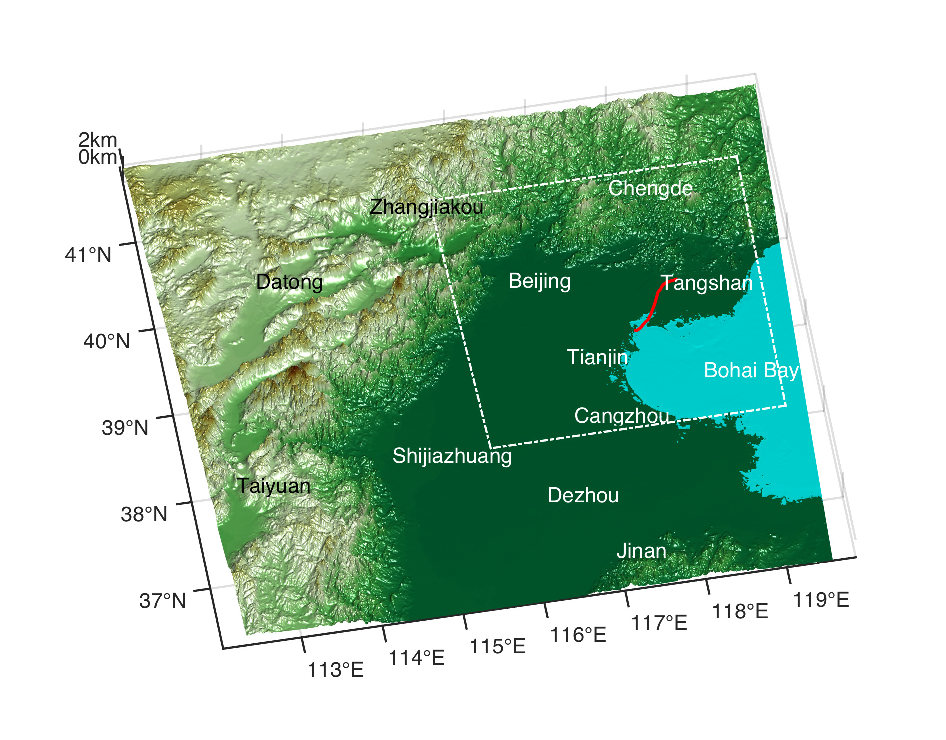
\includegraphics[height=2.5in]{GeoMapTangshan.pdf}
        \caption{唐山地震模拟区域。}
    \end{subfigure}%
    ~
    \begin{subfigure}[b]{0.5\textwidth}
        \centering
        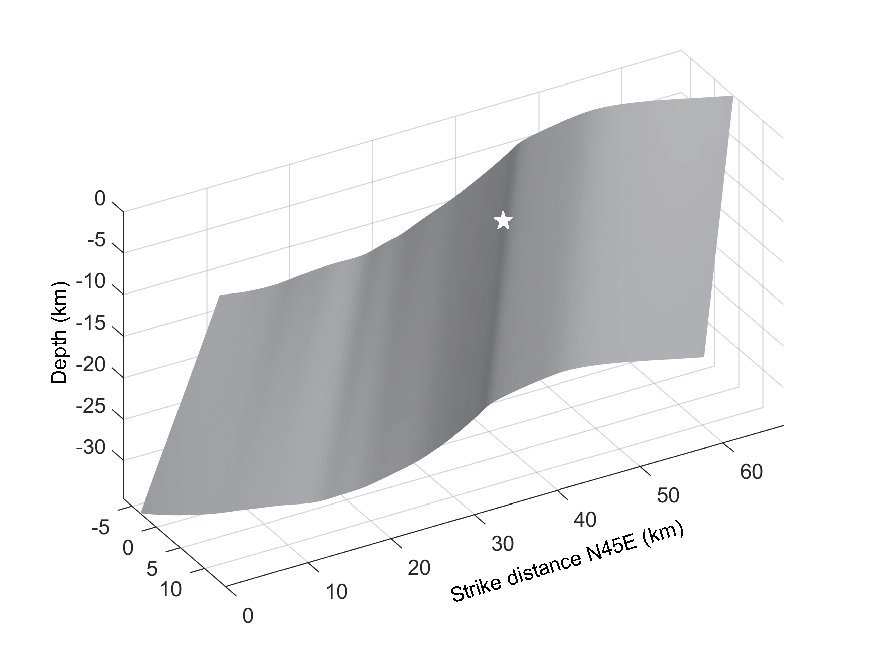
\includegraphics[height=2.5in]{fault.pdf}
        \caption{唐山地震破裂带。}
    \end{subfigure}
    \caption{唐山地震模拟区域和地震破裂带。}
    \label{fig:tangshan_region}
\end{figure}


在未使用实时压缩策略的情况下,非线性唐山大地震模拟的峰值性能为15 PFlops,添加了实时压缩方案后非线性唐山大地震的峰值性能高达18.9 PFlops。距本文作者所示,这是目前世界上最大规模的非线性地震模拟,而模拟的频率和分辨率也是在同等模拟规模下达到最高。唐山地震的塑性地震动模拟首次使我们能够定量估计唐山地震灾区的危害,为华北地区建筑物的抗震工程的标准设计提供指导。

值得一提的是,尽管神威超算的字节浮点比例(byte-to-float rate)只有美国泰坦(Titan)超算的五分之一,但是本研究所达到的计算效率高达15%,超过了以前在Titan \citep{roten2016high}上所获得的效率——11.8%。

\subsection{完整的地震模拟框架}
完整的大规模地震模拟工作流程十分复杂,本研究采用模块化的方式开发了不同的组件,并设计良好的接口,将不同的组件耦合成统一的地震模拟软件框架(如图\ref{fig:framework}所示)。它包括动态破裂震源生成器模块、地震波波场传播模块、三维模型插值与划分模块、震源划分模块、波场快照输出和重启模块。不同模块的的设计原则如下:
\begin{itemize}
  \item 动态破裂震源生成和地震波波场传播模块:地震模拟中计算量最密集的模块。首要考虑该模块代码的可扩展性,使其能够高效扩展到神威超算百万甚至上千万核心。其次考虑每个核心代码的运算效率,高效的有限差分运算是地震波传播的关键;
  \item 三维震源划分、模型插值/划分模块:地震模拟的预处理模块。根据动态破裂震源生成和地震波波场传播模块在不同平台的实现,对震源和模型进行划分和插值。通过预处理,耦合动态破裂震源器和地震波波场传播模块。并以最适合特定超算平台的IO、内存、通信方式,为地震波传播模块提供输出;
  \item 波场快照输出模块与重启模块:地震模拟后处理模块。为了提高地震波波场传播模块的效率,地震波传播模块以最高效的方式将波场快照和重启参数输出到磁盘中,波场快照输出模块与重启模块再对输出的数据进行再处理,形成最终结果。
\end{itemize}

虽然高效的有限差分运算代码是提升地震波模拟性能的关键,但当计算规模扩展到成千上万甚至十几万进程时,通信和IO环节变得同样重要甚至更重要。因此将涉及不同资源(计算、通信、IO)的任务进行模块化处理,并集成到统一的软件框架中,是运行大规模地震模拟的基础。

\begin{figure}[ht]
\centering
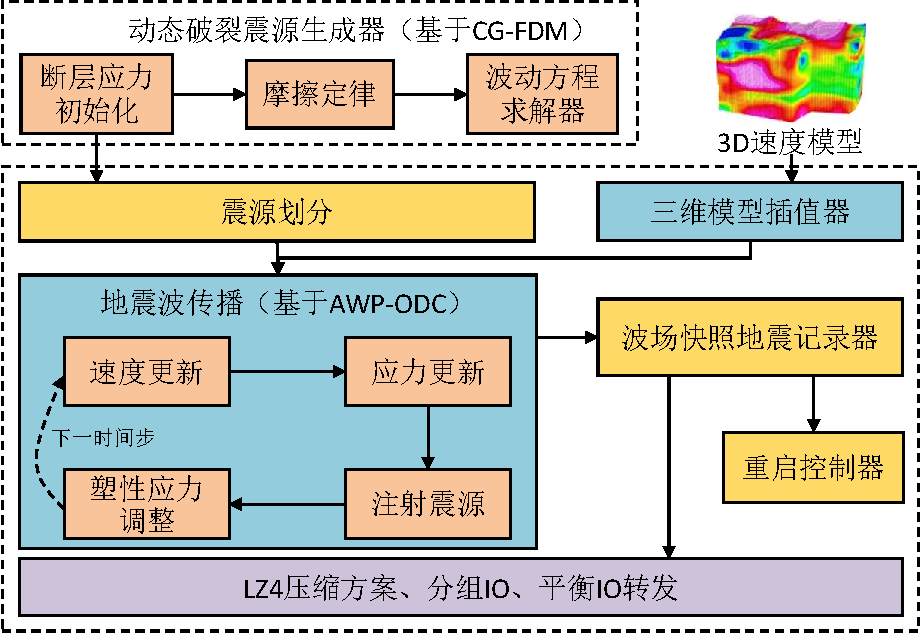
\includegraphics[width=0.9\columnwidth]{地震框架-crop.pdf}
\caption{基于太湖之光的统一地震模拟软件框架。该框架由动态破裂震源生成器、数值计算网格的生成器、地震波传播模块以及其他辅助模块组成。}
\label{fig:framework}
\end{figure}

\subsubsection{动态破裂震源生成与地震波波场传播模块}

软件框架中的动态破裂生成模块基于CG-FDM软件\citep{zhang2014three}进行二次开发而成。该模块具有初始化断层应力、执行摩擦定律控制以及通过波传播生成震源的功能。动态破裂震源生成器的输出是地震破裂震源,并作为地震波传播模块的输入。地震波传播模块基于AWP-ODC \citep {cui2010scalable},并针对太湖之光的特殊体系结构进行了全新的设计。这个模块占据了大部分计算时间,也是并行优化和创新的重点。地震波传播的核心计算是求解速度-应力张量方程,主要流程包括:速度更新、应力更新、震源注入和塑性应力调整。

图~\ref{fig:awp-workflow}描述了地震模拟的核心计算流程。每一个计算核心(kernels)都几乎涵盖了20-40个三维网格,其中大部分网格的大小相同。为了支持这样复杂的工作流程,特别是为了促进未来可能的算法调整,在我们的重新设计和移植过程中,我们将每个内核封装为一个标准模块,可以轻松地与其他模块通过接口进行衔接。

\begin{figure}[ht]
\centering
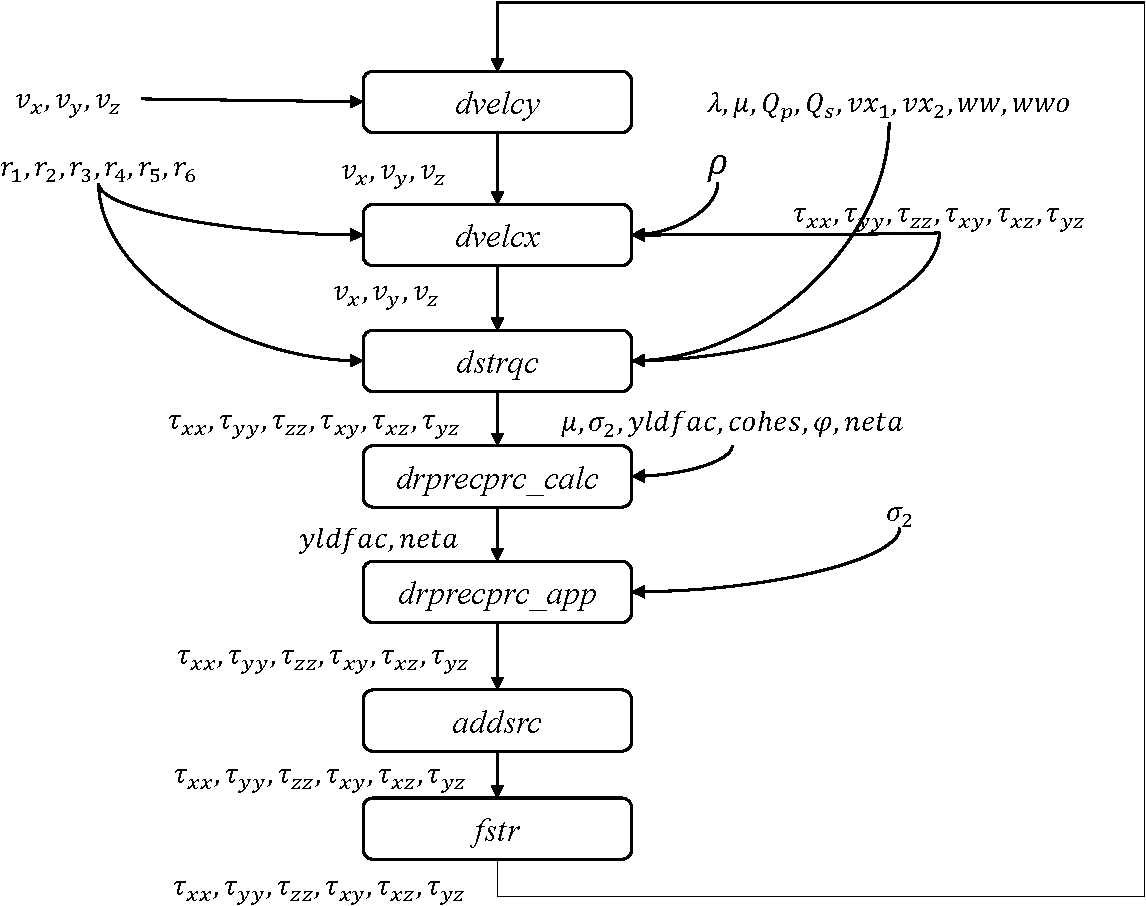
\includegraphics[width=0.8\columnwidth]{AWP流程图-crop.pdf}
\caption{地震模拟的核心计算流程,其中变量以数组表示,计算以kernel表示。}
\label{fig:awp-workflow}
\end{figure}

在一次典型的地震模拟中,每一个迭代步的工作流程由以下五个主要步骤组成:

\begin{itemize}
\item {\bf velocity update}:基于上一个时间步的速度和应力数组,完成速度的更新,包括Halo区域 (由kernel $dvelcy$完成)和中心区域(由kernel $dvelcx$ 完成)。

\item {\bf stress update}:使用速度,应力阵列,Lam系数和频率相关的地震波震级衰减参数Q等等数组来计算Halo区域和中心的应力更新(kernel $dstrqc$);

\item {\bf stress adjustment for the fault}:检查屈服应力是否越界(kernel $drprecprc\_calc$),并对断层区域进行相应的调整(kernel $drprecprc\_app$);

\item {\bf injection of source}:注入震源(kernel $addsrc$)来更新当前时间步的波场。

\item {\bf stress adjustment for the free surface}:对自由边界进行应力调整(kernel $fstr$)。
\end{itemize}

以上描述的每一个步骤都涉及到了大量的大型三维数组读写。尽管每个内核都涉及高密度的算术运算,在太湖之光超算上性能的主要限制条件却来自于内存带宽的瓶颈。


\subsubsection{并行震源划分与介质模型插值模块}
\label{sub:并行震源划分与介质模型插值模块}
在大规模地震模拟中,当震源和介质模型的文件规模逐渐上升到TB量级,地震模拟的预处理也逐渐成为整个软件的瓶颈,耗时不断上升,甚至因为资源不足导致程序无法运行。因此打造高效和高可扩展性的震源、模型划分软件是大规模地震模拟必要过程。本研究采用两种划分方式对震源进行划分:多进程串行划分方法和并行MPI-IO划分方法。

多进程串行划分方法按照既定的地震波传播并行划分规则,将单一的大型震源针对每个进程所处理的区域划分成若干小型震源,并输出到不同的文件中。这种方法能够充分利用神威超算系统的IO带宽。但是,由于动态破裂震源通常为模拟区域内的一个小范围曲面,因此震源位置非常集中,在划分的过程中会出现严重负载不均衡问题,降低了运行效率。此外,在震源震动时间通常较长的情况下,加上过度集中的震源,很容易导致单进程所需的内存超过系统最大内存。本研究在按空间划分的基础上再按照时间进行划分,有效的避免了划分时部分进程内存不足问题。

并行MPI-IO方法并不对大震源物理切分成若干个小文件,而是在地震传播模块中采用并行MPI-IO接口读取大震源的不同部分。理论上,MPI-IO库在调用良好的情况下能够提供可观的带宽和扩展性,但在神威超算系统中,并行MPI-IO接口却展现出非常糟糕的带宽和扩展性。这是移植的MPI-IO接口并没有在神威超算特殊的片上异构众核架构中深度从核优化。

因此从效率和可扩展性出发,并行震源划分采用了多进程串行划分方法。虽然该划分方法会导致了负载不均衡,但划分过程的效率主要取决了IO带宽,处理密集震源的核心几乎能够利用全部IO带宽,因此并不会因为负载不均衡而严重影响效率。

实际介质模型通常不大,在进行多尺度地震模拟时,介质模型按照地震模拟的网格分辨率进行插值,得到新的介质模型。在大规模地震模拟中,再使用并行划分方法为每个进程构建输入。通过简化流程,提高效率,本研究直接在地震波传播模块中集成插值模块,将实际介质模块插值得到目标模型,好处是无须将完整的介质存储到磁盘。

\subsubsection{波场快照输出与重启模块}
地震波波场快照是地震波模拟的结果,是可视化的必要输入数据。本研究提供了灵活的波场快照输出方式,用户可以指定任意范围任何分辨率的波场快照,且同时支持多尺度波场快照输出。低分辨率的波场快照可用于地震模拟可视化,高分辨率的波场和地震记录可精细分析地面运动和烈度。

大规模的地震模拟伴随着巨大的计算量,即便拥有大型超算的支持,计算时间仍然可能需要十几个小时甚至几十个小时。更多计算核心的参与也意味着发生硬件和软件错误的概率更大。这种情况下,软件的容错能力则显得非常重要。例如,在神威超算全机模拟中,有超过一千万核心参与运算,四小时内发生几乎会发生一次硬件或软件错误,如果没有容错机制,整个地震模拟过程需要重头开始,严重地浪费了之前四小时的计算。不具备容错机制几乎无法完成需要长达十几个小时才能完成的模拟。本研究设计了重启模块,在地震波传播过程中,周期性地将每个进程的内部状态变量存储到硬盘中(检查点)。当程序异常退出时,地震模拟可从最近的检查点启动,继续模拟。

在波场快照输出与重启模块中,IO是影响最大的因素。例如在16米分辨率下,每个重启检查点需输出的内部状态变量超过108 TB,这对超算系统的存储带宽和容量都是巨大的挑战。本文使用与第\ref{sub:并行震源划分与介质模型插值模块}节类似的多进程串行输出方法,每个进程将各自的串行输出到硬盘中,并调用后处理程序对数据进行合并。此外,我们还采用了LZ4压缩方法以降低输出数据量,降低存储开销,并采用诸如“组I/O”和“平衡I/O转发”等技术,实现了120GB/s的峰值I/O带宽,达到了该文件系统峰值带宽的92.3%。

\subsection{性能与扩展性}

\subsubsection{如何测量性能}

地震模拟的性能通过每秒钟浮点运算次数(FLOPS)来衡量。地震模拟的主要运行时间是地震波正演模块,初始化的时间可以忽略不计。对于核心计算时间,本研究通过记录记录运行100个时间步所花费的时间来计算每一个时间步所花费的平均时间。值得注意的是此处并不包含IO时间,因为在大规模地震模拟中,IO时间占比较小(不考虑重启)。

本文研究使用两种方法来测量浮点数运算次数,分别是数汇编代码中的所有浮点运算指令以及使用太湖之光编译器辅助的硬件性能监视器PERF工具。这两种方法都产生了类似的浮点数操作次数。本研究使用PERF工具来测量本程序所执行的平均浮点运算。为了更加公平地与其他类似工作做对比,本研究为优化而添加的所有额外操作(例如压缩相关操作)都不计入浮点次数。

\subsubsection{计算核心优化结果}

正演算法的计算热点比较集中,主要为速度更新和应力更新两个核函数。对于速度物理量的更新,计算中心区域和Halo区域的核函数$ dvelcx,dvelcy $是计算量最大的两个计算核心。对于应力物理量的更新,$ dstrqc $是计算量最大的计算核心。对于塑性部分,$ drprecprc\_calc $是整个程序中最耗时的部分。剩下的内核包括$ fstr $,$ drprecprc\_app $,MPI的预处理和后处理($ unpack\_VY $,
$ gather\_VX $和$ unpack\_VX $),这消耗了总运行时间的1-2%。本研究对上述的核函数都进行了极致的优化,以便实现最高的性能。

图~\ref{fig:kernel-result}演示了当采用不同的优化方法时,这些不同计算核心的性能和带宽改进结果。可以看到,几乎所有的核函数经过优化后都获得了30倍左右的性能加速比,并且DMA传输带宽达到了总带宽的70%到80%左右。唯一的例外是$ fstr $核函数,$fstr$核函数的计算密度很低,内存访问不规整,只实现4倍至5倍的加速。从图~\ref{fig:kernel-result}还可看到,经过了一系列的优化后,不同核函数优化前和优化后在总执行时间内的耗时分布并无太大变化。

\begin{figure}[t]
\centering
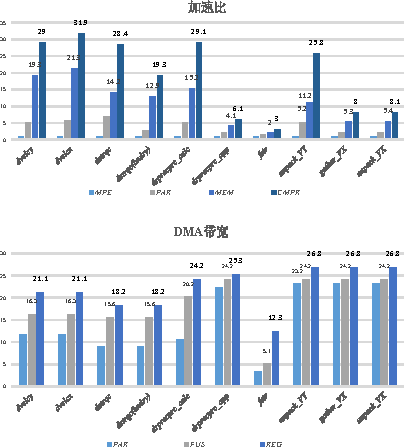
\includegraphics[width=0.9\columnwidth]{AWP-performance-crop.pdf}
\caption{地震模拟中不同计算核函数采用了不同优化技术的加速比和内存带宽。 `MPE'代表仅使用主核的原始版本。 `PAR'是指使用了多层级并行划分方案并使用了64个从核并行计算的版本。 `MEM'是指采用所有与内存相关的优化的版本。 “CMPR”是指进一步应用即时压缩方案的版本。}
\label{fig:kernel-result}
\end{figure}

在不同的优化方案中,内存相关的优化效果最明显,其中共位数组融合优化方案起着最重要的作用。图\ref{fig:fusioncmp}展示了在最核心的$dvelcx$和$dstrqc$核函数中共位数组融合的前后对比图。使用共位数组融合,最耗时的核函数的性能提升了4倍。

\begin{figure}[ht]
\centering
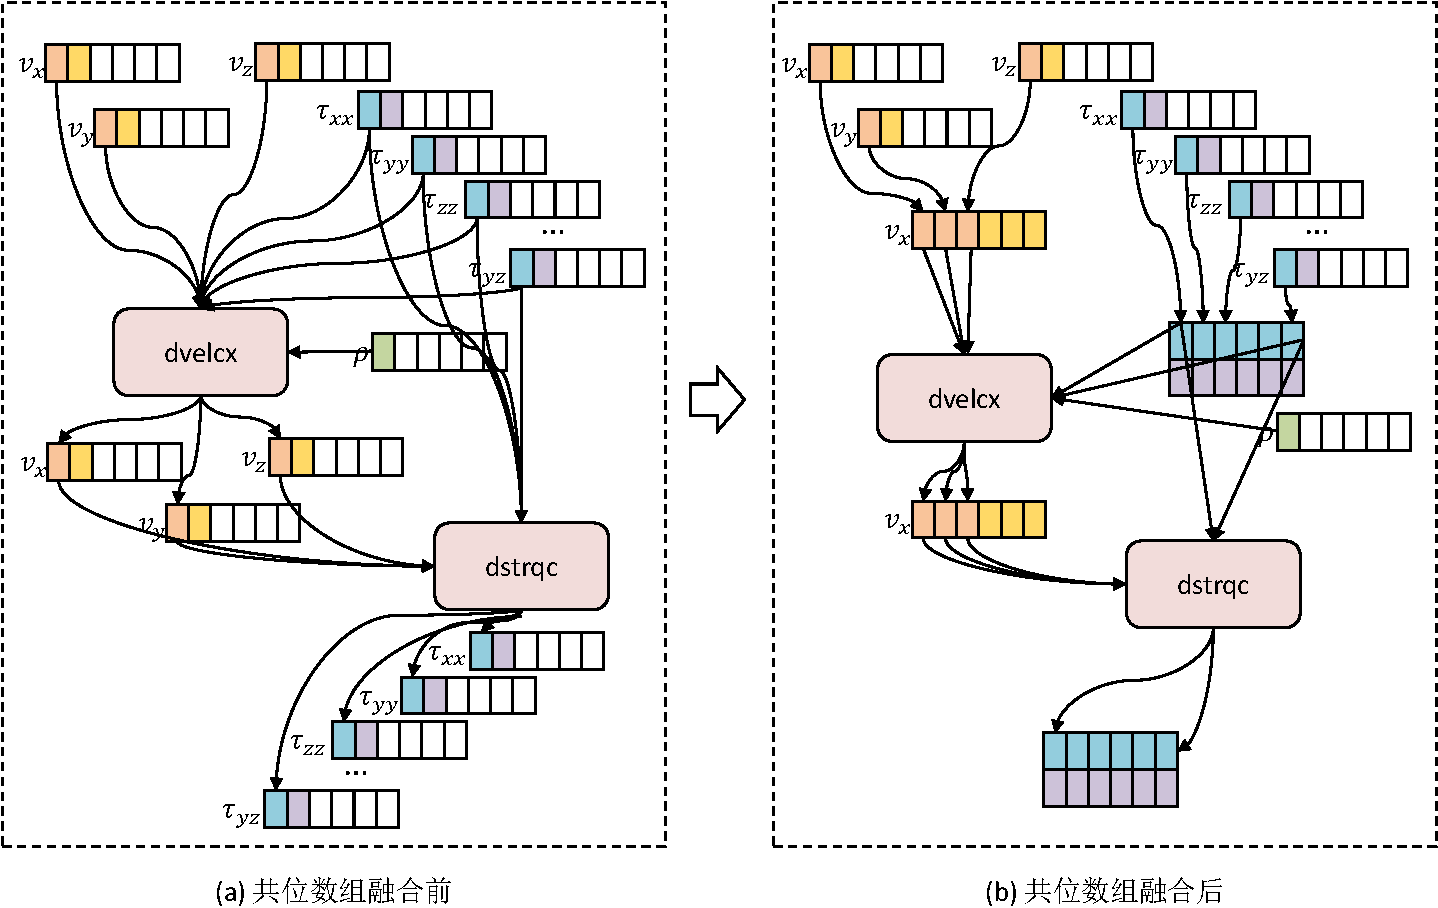
\includegraphics[width=0.9\columnwidth]{figures/数组融合前后对比-crop.pdf}
\caption{共位数组融合前后对比图。}
\label{fig:fusioncmp}
\end{figure}

\subsubsection{压缩方案精度结果}


为了验证压缩方案的准确性,本文工作比较了在不同分辨率下使用压缩方案和不使用压缩方案的仿真结果。图\ref {fig:compress_valid}对比了宁河和沧州两个台站压缩前后地震记录。宁河县位于唐山地震断层附近,在地震期间承受了巨大的破坏。图中的蓝色实线是未压缩的结果,红色的虚线是压缩的结果,可见红线和蓝线的波峰波谷位置几乎相同。由于有损压缩算法经过多次迭代后精度有所损失,红线尾波处虽不能完美匹配蓝线,但仍保留了大量细节,这对于大规模地震模拟而言已经精确。


\begin{figure}[ht]
\centering
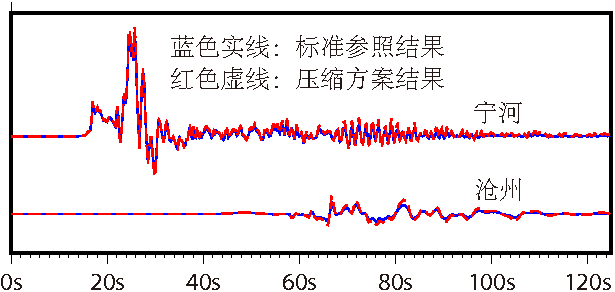
\includegraphics[width=0.8\columnwidth]{CompareCompress-crop.pdf}
\caption{500米分辨率下唐山地震模拟压缩方案验证。}
\label{fig:compress_valid}
\end{figure}

沧州站离震中较远,地震波需经过较长时间传播才到达。由于经过前期较长时间的传播和压缩误差积累,红线和蓝线的波峰波谷并没有完全匹配。但对于此类情况,压缩后的结果可以承受稍微较高的精度损失。从图中可见,直到120秒仿真结束时,两条曲线仍可以很好地匹配。比较结果表明,虽然压缩在一定程度上引入了误差,但实际中仍可使用这套实时压缩方案。它不仅能获得更好的性能,还能进行更大规模的地震模拟。

\subsubsection{弱扩展性结果}

弱扩展性表示当计算规模和计算核心同时增大时计算能力的变化。图~\ref {fig:weak-scaling}描述了线性和非线性情况下的地震模拟程序的弱扩展性结果。 在这两种情况中每个核组计算的网格大小均为$160\times 160$,然后逐渐扩展到整个机器。从8,000个进程到160,000个进程,本研究的大规模唐山大地震模拟实现了97.9\%的并行效率,几乎达到了完美的线性加速效果。这意味着该应用的通信策略非常高效,实现了接近完美的计算通信重叠。

无压缩的线性地震模拟通过使用160,000进程取得了10.7 PFlops的峰值性能。非线性地震模拟具备更密集的计算,取得了峰值性能为15.2 PFlops。采用实时压缩方案后,相同的内存宽能够处理更多的数据,这分别进一步将线性和非线性地震模拟的性能提高至14.2 Pflops和18.9 Pflops。

\begin{figure}[ht]
\centering
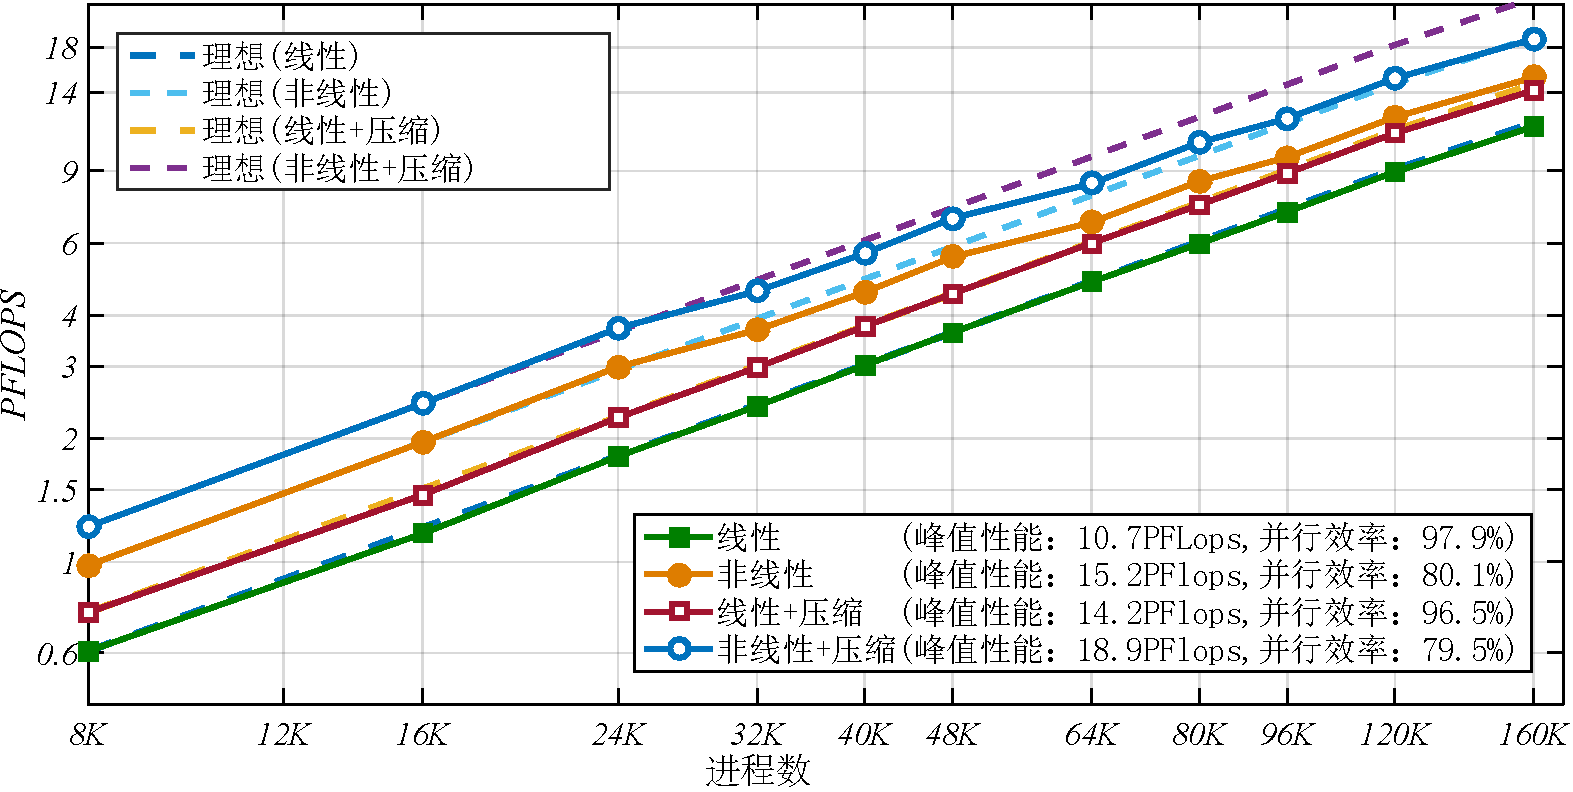
\includegraphics[width=0.9\columnwidth]{weak_scaling.pdf}
\caption{线性和非线性地震模拟的弱扩展性结果。测量的MPI的进程数从8000个扩展到160,000个,其中每个CG对应于一个MPI进程。}
\label{fig:weak-scaling}
\end{figure}

\subsubsection{强扩展性结果}

强扩展性描述了当问题规模不变时,增大计算核心带来的加速比。由于神威超算有40000个节点,测试强扩展性的问题规模太小,则大规模并行时每个节点的任务很小;问题规模太大,则小规模并行时节点内存可能无法容纳子问题。因此本研究针对不同的计算规模设计了三种不同网格大小算例。图~\ref {fig:strong-scaling}显示了基于三种不同网格大小的线性,非线性,含压缩以及不含压缩情况下的强扩展性测试结果。 

由图~\ref {fig:strong-scaling}所知,不管是线性或非线性地震模拟,含压缩或者是不含压缩,本研究的地震模拟都达到了类似的强扩展性结果。但随着进程数量的不断增加,性能出现了下降。本文分析性能的下降是由两个方面造成的:(1)计算与通信的比例减小;(2)外部Halo区域与每个进程内计算的网格体积比例的减小,这降低了AWP软件的计算和通信重叠的效果,使得通信无法完全被计算隐藏。

\begin{figure}[ht]
\centering
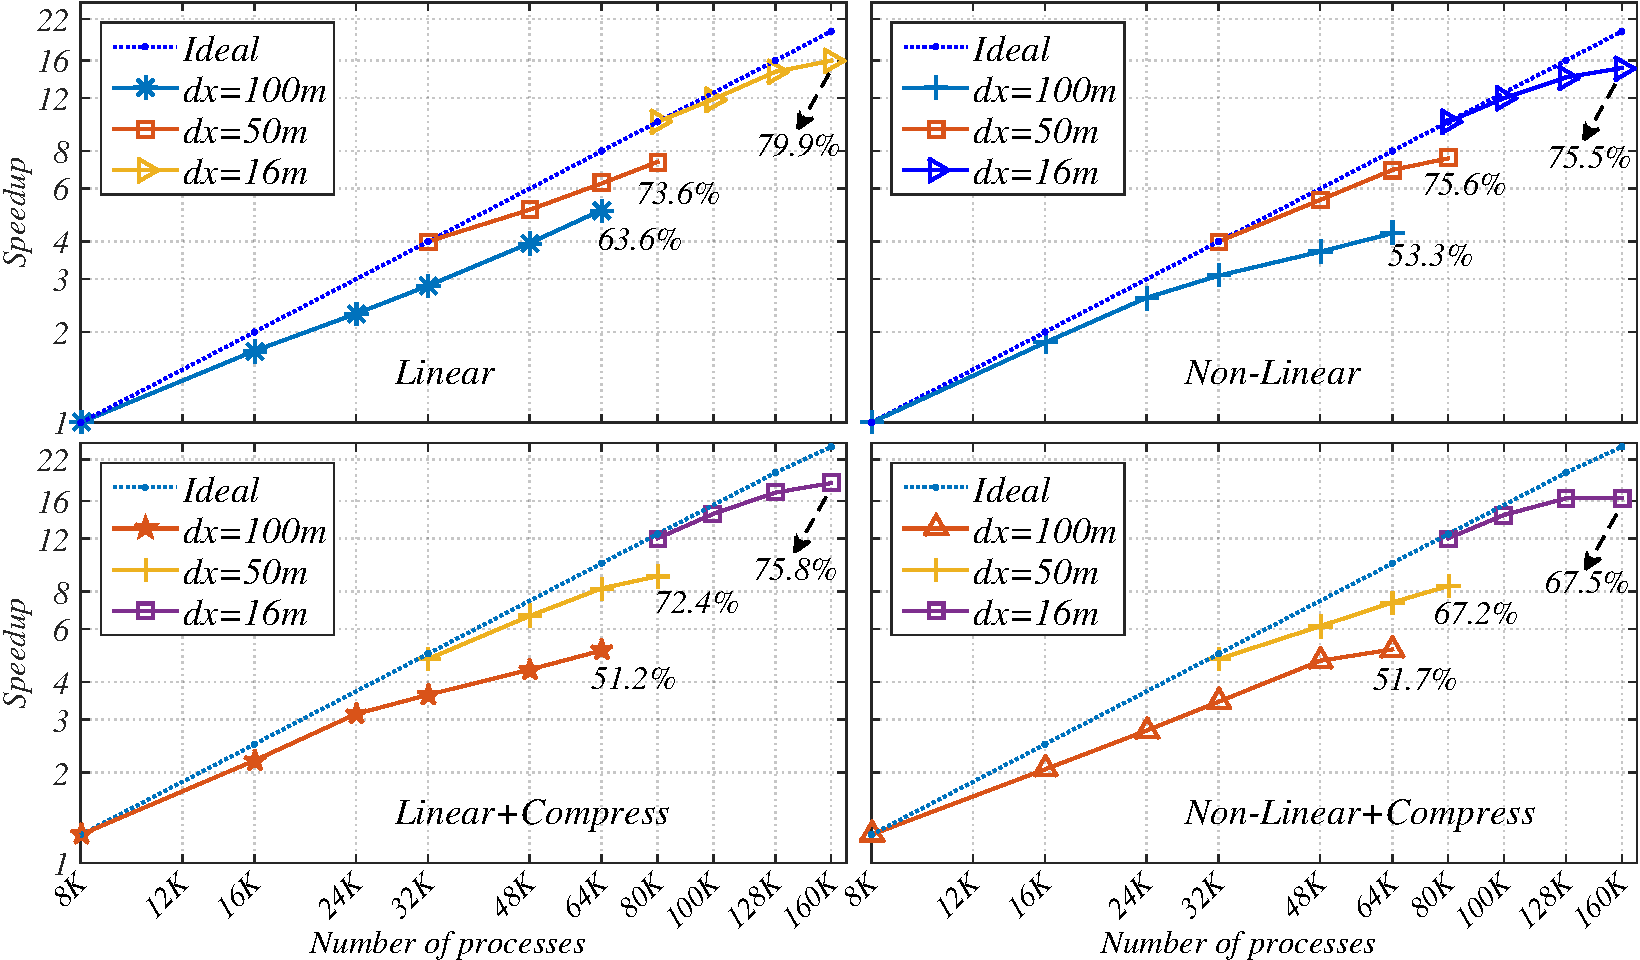
\includegraphics[width=1.0\columnwidth]{strong_scaling.pdf}
\caption{线性和非线性地震模拟在三种不同的问题规模中的强扩展性结果。测量的MPI进程从8,000个扩展到16,000 个,其中每个CG上对应一个MPI进程。}
\label{fig:strong-scaling}
\end{figure}


\subsection{地震模拟结果}

传统对剧烈地震的模拟通常局限于低频信息,因为高频模拟需要计算机提供巨大的内存和强大的计算能力。凭借太湖之光的强大计算能力,本文研究成功模拟了唐山大地震。本次模拟的区域为$320km \times 320km \times 40km$,地震波的最大频率为$18Hz$。本研究的地震模拟利用复杂几何断层引发的破裂动力源来推动地震波传播,估算唐山地震在华北地区的地震危险性分布。唐山断裂的几何构造以及构造应力场是通过观测和合理的推断推导出来的。在动态和地面运动模拟中,实现了水平方向上分辨率为25公里,垂直方向上的分辨率为2公里的华北地区的三维速度模型。通常情况下,沉积结构被添加到强大的地面运动模拟中。这些复杂性的三维模型使我们对唐山地震的模拟更接近现实。

\subsubsection{动态破裂源}

为了重现由唐山大地震造成的地震灾害,我们需要尽可能准确地描述地震环境和地震过程。地震发生后,唐山市南部出现了8至11公里的地表破裂带。这个破裂带由十多条东北方向的走滑右旋(right-lateral)、走滑左步(left-stepping)梯形断裂构成,总体走向为 N30$^\circ$E,水平方向上的位移为1.5至2.3米,垂直方向上的位移为0.2至0.7米。在地表破裂带的南部,垂直位移从西部上升到东部。在发现新的地表破裂带\citep {Qiu_discovery_2005}之后,更多的地质证据证明,1976年唐山地震的地表破裂带延伸至城市西南部超过47公里 \citep{guo_new_2011},正如图\ref{fig:tangshan_geomap}(a) 所示。此外,深部地震反射剖面表明,唐山断裂系统极为复杂,可能深入到莫霍界面\citep{liu_seismogenic_2007}。

根据之前对唐山地震的调查和观测,本文研究构建了唐山断裂的三维几何结构,如图\ref{fig:tangshan_geomap}b 所示。非平面断层分别沿着走向(strike)和倾向(dip)方向延伸约70公里和35公里。两个水平准则的压缩应力与图\ref{fig:tangshan_geomap}(a) 所示的方向一样用作动力学模拟中的驱动力。

描述断层几何的复杂性需要强大的数值方法和计算能力才能实现不规则断层面上的动态条件。我们在太湖之光超级计算机上面进行了基于复杂几何断层的唐山大地震动力破裂模拟,这为后续的地震波传播模拟提供了震源。图 \ref{fig:tangshan_geomap}(b) 表示了 T=10.5s 时唐山地震破裂的绝对滑动速率(absolute slip rate)快照。由于断层走向的曲率变动的原因,破裂断层的东北侧表现出更多的复杂性。这证实了动态破裂模拟过程中复杂三维断层几何的重要性。

\begin{figure}[t]
\begin{tabular}{cc}
(a) & (b) \\
    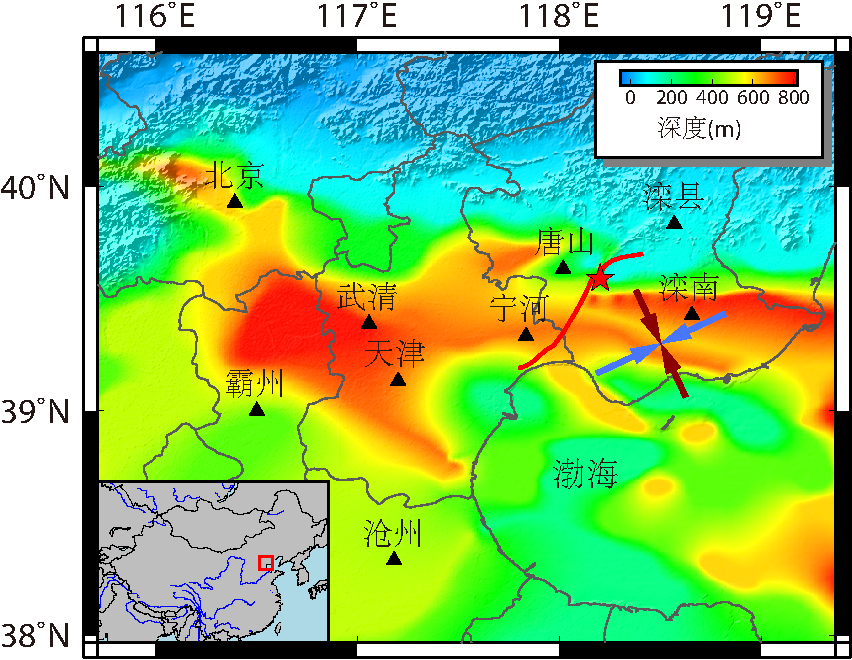
\includegraphics[width=0.5\columnwidth]{Tangshan_geomap-crop.pdf} &
    \includegraphics[width=0.5\columnwidth]{Tangshan_Fault1.eps}
\end{tabular}
    \caption{
(a)唐山地震模拟的强地面运动,模拟的区域为$320km \times 320km \times 40km$。 该地区的沉积深度以不同颜色表示了震中(红星),地震断层(红色曲线)和应力场(红色和蓝色矢量)。 (b)通过CG-FDM方法计算的动态源(T=10.5s 时的断层的绝对滑移率。}
    \label{fig:tangshan_geomap}
\end{figure}


\subsubsection{强地面运动}

由于动态破裂、复杂的三维介质和地质结构,地震可能产生高频能量(高达至少10 Hz)。因此具有高效的高频分量的地震图是工程地震分析的重要数据,能够为建筑物的抗震设计提供了合适的标准。

\begin{figure*}[ht]
    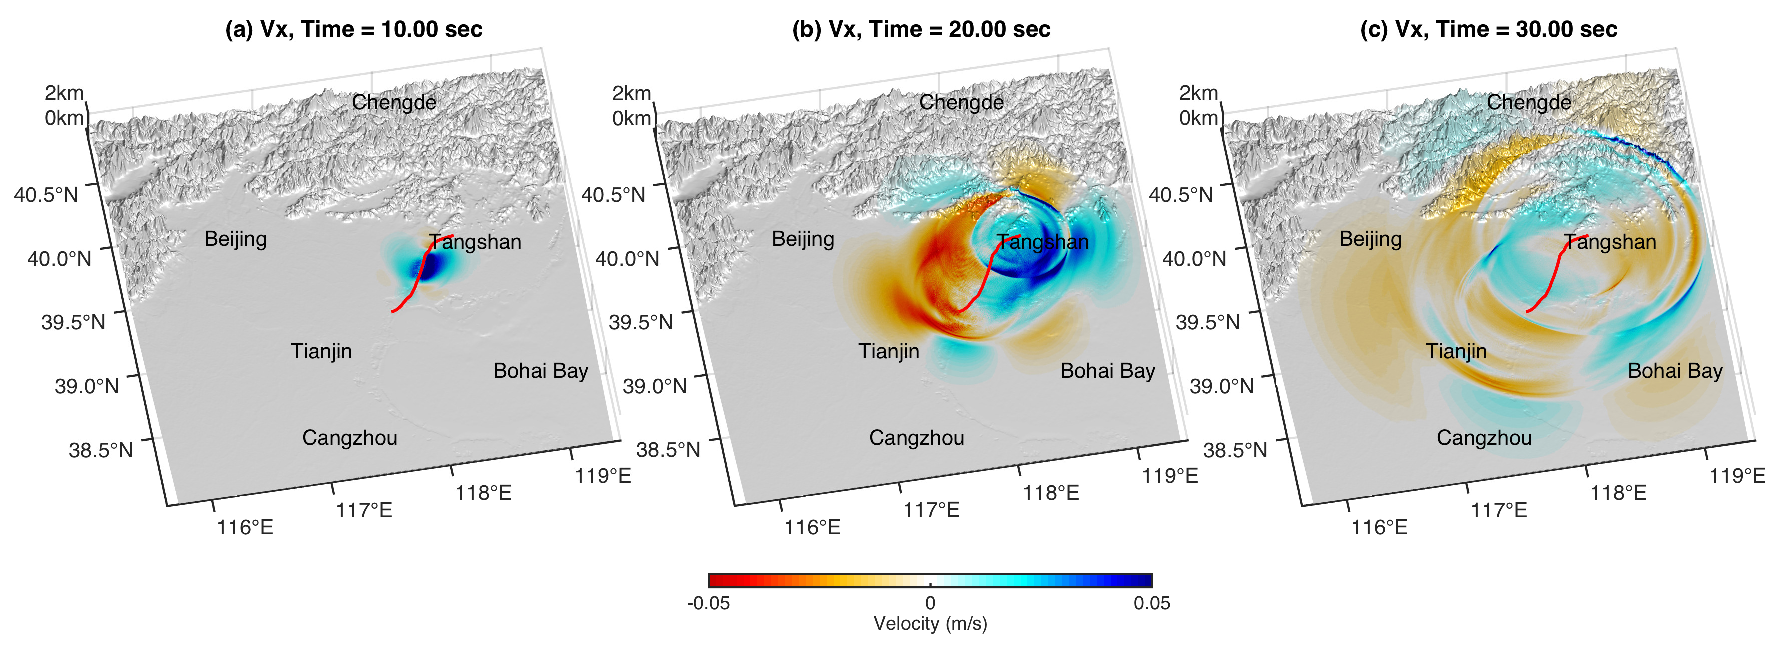
\includegraphics[width=1.0\columnwidth]{Snap_Vx_tangshan.pdf}\\
    \caption{速度分量(东西方向)分别在(a)T = 10s,(b)T = 20s,(c)T = 30s等不同时刻地震波传播的波场快照。}
    \label{fig:strong_motion_2}
\end{figure*}

图\ref{fig:strong_motion_2}描述了在(a)T = 10s,(b)T = 20s,(c)T = 30s等不同时刻地震波传播的波场快照。破裂从断层中心开始,向双向传播。 由于近地表的弯曲断层,北方波场显示出更复杂的模式,这表明了大地震模拟期间非平面断层几何的重要性。

\begin{figure}[t]
  \centering
  \includegraphics[width=1.0\columnwidth]{CompareDifferentSpatialResolution-crop.pdf}
  \caption{
不同空间分辨率的地震模拟结果比较。左栏是空间分辨率为200m的地震模拟,右栏相应的16m分辨率。 (a $ \thicksim $ b)宁河县和沧州市速度(W-E分量)地震记录图; (c $ \thicksim $ d)地震发生后60s处的速度场快照,右上角的缩放子图描述了含有沉积作用的区域的细节(虚线方框);(e $ \thicksim $ f)地震震害分布图,由水平方向上的地面峰值速度计算获得。}
  \label{fig:strong_motion}
\end{figure}

如图\ref{fig:strong_motion}a$\sim$b 所示,不同的空间分辨率模拟之间存在明显的差异,较低的空间分辨率(如200m)不足以准确地描述盆地结构,如图\ref{fig:tangshan_geomap}(a) 所示,其中最大沉积深度为800米。

因此严格来说,使用较低的空间分辨率来计算尾波是不准确的。本研究的使用高分辨率进行模拟可以看到沧州市主要地震能量在较高空间分辨率下模拟的尾波振动比较低,如图\ref{fig:strong_motion}(b)所示。此外,由于唐山地震的震中位于沉积盆地,地震的主峰甚至无法准确计算出来(见图\ref{fig:strong_motion}a$\sim$b,宁河)。总而言之,空间分辨率的高低直接关系着复杂地震模拟的准确度,16m以上的高分辨率模拟是三维复杂结构的地震模拟的关键。

本文研究还比较了地震波波场快照和震害图(hazard map)来说明不同结果的细节。 图\ref{fig:strong_motion}c$\sim$d 描述了唐山地震发生60s后地震波波场的快照。 虽然波场的主要行为是相似的,但在小尺度上出现了明显的差异。 图\ref{fig:strong_motion}c$\sim$d右上角的放大图片说明了这次地震中的沉积物效应,可以看到在空间低分辨率下沉积物效应不能很好地被描述出来。

唐山地震的震害图可以通过计算水平方向上的地面峰值速度来获得。本文研究比较了200m和16m分辨率下的震害图(如图\ref{fig:strong_motion}e$\sim$f 所示)。其中红色(烈度为9$\sim$11)表示地震中最严重的破坏,这非常依赖破裂断层的位置。但由于沉积作用,高强度的破坏影响被重新分配了:位于唐山市的滦南县虽然不在地震断层的周围,也遭受了严重的破坏。对于不同的分辨率下地震模拟结果,震害图显示了高分辨率模拟(如图\ref{fig:strong_motion}f 所示)和低分辨率模拟(如图\ref{fig:strong_motion}e 所示)的巨大差异。例如,武清地区的烈度在左图中为6级(蓝色),右图为7级(绿色)。这再次证明了高分辨率模拟在实现准确地震危险图方面的重要性。

% \section{汶川大地震模拟}
% \section{集合全波形反演}
% \section{本章小结}

% \section{总结}

% 我们在这里要强调的一个信息是,本研究设法将太湖之光超级计算机的各个方面的性能都发挥到了极限。 如Table \ref{tb:push-limit}所示,对于每一项指标,我们都几乎将其发挥到了极限,特别是对于内存系统。 因此,即便太湖之光超算系统的内存系统与美国的泰坦超算系统相比处于劣势(太湖之光的byte-to-float之比仅为美国泰坦超算的1/5,而每个计算密集的kernel需要30个3D数组),我们仍然能够在不使用压缩方案的情况下使用太湖之光的10,400,000个计算核心,实现了性能为15.2-Pflops非线性唐山大地震模拟,达到了全机峰值性能的12.2%。

% \begin{table}[!t]
% %\footnotesize
% \caption{
% 太湖之光能够支持的最大地震模拟测试用例下的计算与内存性能(无压缩情况下)。此处描述的是每个核组的计算性能,内存大小和带宽;单个CPE从核的LDM大小。请注意,在每个核组的8 GB内存中,我们必须为整个机器的正常运行和MPI缓冲区预留2.5 GB的空间。}
% \label{tb:push-limit}
% \centering
% \begin{tabular}{cccc}
% \hline\hline
%   & Effectively used & Peak & \% \\

%   Computing Performance & 98.7 Gflops & 765 Gflops & 12.9\% \\
%   Memory Size & 5.2 GB & 5.5 GB & 94.5\% \\
%   Memory Bandwidth & 25 GB/s & 34 GB/s & 73.5\% \\
%   LDM Size & 60 KB & 64 KB & 93.8\% \\\hline
% \hline
% \end{tabular}
% \end{table}

% 更令人兴奋的创新当然是实时压缩方案,它以可接受的准确度损失为代价,将我们的仿真性能和功能扩展到超出机器物理约束的范围。 通过利用10,485,760个CPE进行神威超算整机模拟,并且采用实时压缩策略,本研究的模拟规模相当于使用两台神威超算进行的模拟,这几乎是历史上最大规模的一次科学计算数值模拟。采用实时压缩方案,我们获得了两个好处,在物理内存限制的情况下能够进行更大规模的科学模拟,或者在相同的问题规模下,将地震模拟的性能进一步提升了24%。我们的压缩方案将我们的计算性能扩展到了18.9 Pflops(峰值的15%),并且使我们能够支持18 Hz、8米分辨率的地震模拟。这对于以前的技术水平来说是一个巨大的飞跃。 虽然目前的压缩方案主要是针对我们的特定应用和神威架构定制的,但我们相信这个想法有很大的潜力应用于其他应用和其他架构,特别是在内存带宽成为主要限制的时代。
% chapter 非线性唐山大地震模拟 (end)

\section{石油勘探全波形反演成像} % (fold)

人工地震常用于研究天然地震原因和探测当地矿产资源,是地球物理勘探过程中必不可少的手段。石油勘探地震资料处理的方法包括正演和反演方法。正演为了仿真物理过程,在给定的模型下计算合成地震记录;反演的目的是地下结构成像,计算地底矿产资源的分布。本小节以石油物探领域典型的$Marmousi$模型为例,探究集合全波形反演方法在神威太湖之光上的优化效果和成像结果。

\subsection{基于神威超算的集合全波形反演方法}

集合全波形反演方法的热点和函数是正演计算,因此前文研究的所有针对正演优化方法均可用于集合全波形反演方法中。本研究设计的基于神威超算的集合全波形反演方法的计算流程如图\ref{fig:enfwi-flow}所示。

\begin{figure}[ht]
\centering
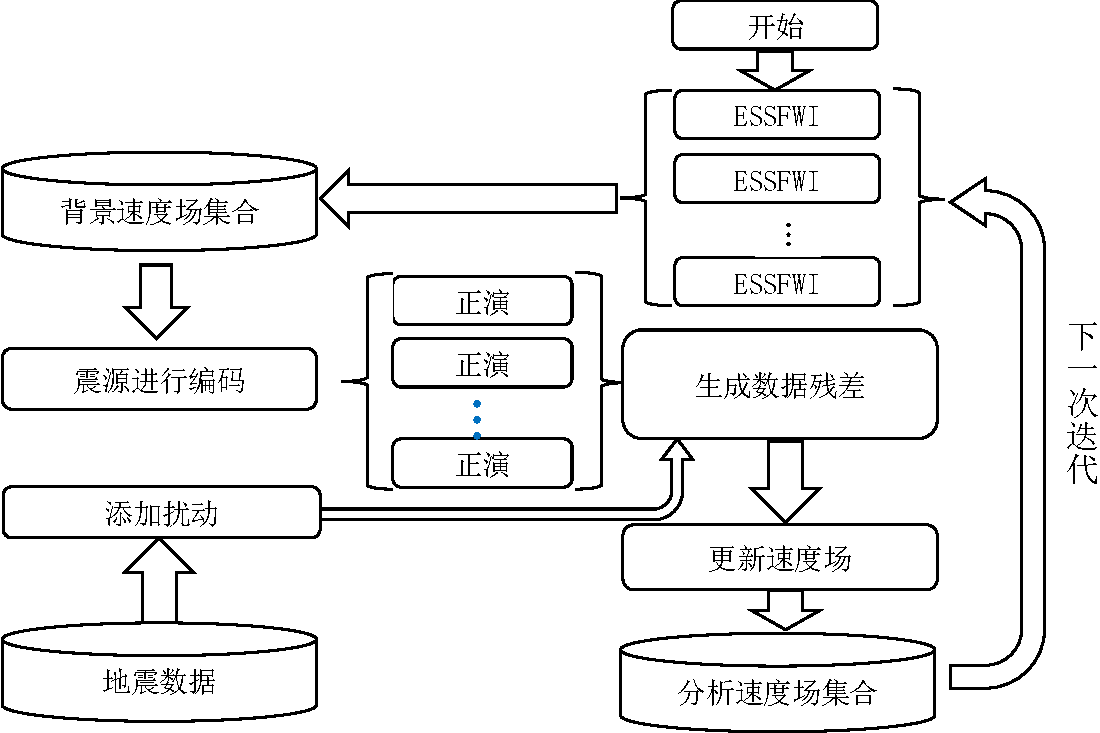
\includegraphics[width=0.9\columnwidth]{enfwi流程图-crop.pdf}
\caption{集合全波形反演算法计算流程}
\label{fig:enfwi-flow}
\end{figure}

采用上文介绍的多层级划分方案、最小DMA数据传输总量推导、寄存器通信等等优化策略,本研究在太湖之光上实现了二维和三维的集合全波形反演应用的主核和从核版本,并基于集合样本和波场区域分解将应用扩展到了8192个进程,充分地利用了太湖之光的大规模计算能力。

神威超算的主核的主频低、逻辑与计算处理能力较弱,从核又无法为主核分担,无法执行通信、IO等操作,性能的瓶颈集中在主核中。因此,本研究尽可能将所有函数移植到从核中,只让主核处理必要的调度、通信、IO等操作。

本文采用了OpenACC和Athread两种并行实现方式,针对不同的函数采取最优的实现。OpenACC具有编程易用性强、开发时间短、可维护性高等优势,集合全波形反演算法中大量的基本向量/矩阵运算如向量/矩阵加法、矩阵/乘法等简单的函数采用了OpenACC并行方法实现。而计算行为较为复杂的函数都采用控制粒度更细的Athread并行方法实现。按照分配线程、DMA数据读取、LDM中数据计算,DMA数据写出流程进行编程实现和性能优化。

在单节点性能取得极致之后我们开始进行多节点并行扩展。本研究中单个样本的速度模型的最大网格大小为$920\times 300 \times 500$,我们按照$8\times 2 \times 4$进行划分以获得接近立方体的子网格,每个子网格的大小为$115\times150\times125$。每个子网格分配给一个MPI进程。集合的样本数目为128个,总MPI进程数到到8192。

由于本实验反演的是中小规模的地质模型,因此并未将太湖之光的所有计算资源充分利用。但本研究为太湖之光定制的集合全波形反演应用是面向大规模三维反演成像设计的,因此充分具备反演大规模模型的能力。

\subsection{性能优化结果}

本小节展示在太湖之光超算平台上针对集合全波形反演应用进行性能优化的结果。图\ref{fig:集合全波形反演算法核心函数从核优化加速比}表示集合全波形反演算法核心函数从核优化加速比。\emph{Intel单核}表示该函数在Intel Xeon E5-2697v2(主频为2.7GHz)机器的性能。为了进行更加公平的对比,Intel平台的结果也是经过深度优化的,包括向量化、缓存分化快(cache blocking)、循环展开等等。\emph{主核}表示神威主核的性能,这是作为比较的基准。\emph{64从核}表示使用64个从核进行深度优化后的性能。

从图\ref{fig:集合全波形反演算法核心函数从核优化加速比}可知,Intel单核性能普遍为神威主核性能的4倍,其中重要的原因是Intel的主频较高。经过64个从核优化之后,不同函数的加速比分布在$6.5\times$至$32.3\times$。性能最好的$fd2t10s$函数取得了32.3倍的加速。这个函数是空间10阶、时间2阶的有限差分运算的核心函数,同时也是$fwd\_prop$、$back\_prop$、$cal\_steplen$等函数的核心子函数。因此,在深度优化$fd2t10s$之后,$fwd\_prop$、$back\_prop$、$cal\_steplen$等函数也相应获得了21至28倍的性能提升。

使用64个从核加速仅获得不足30倍的加速比,效率不足50\%,这似乎不是令人激动的数字。然而当我们对有限差分算法进行深入分析之后发现,空间为10阶的中心stencil运算是严重的访存受限问题,性能的提升取决于数据的复用以及对访存带宽的利用率。经过我们的细致优化(包括多层级数据划分、数组融合、寄存器通信,从核ID重映射、内存字节对齐等等),$fd2t10s$函数的DMAD带宽效率达到了26GB/s,达到了神威单核组的访存峰值带宽的74\%,在有限的LDM中,这几乎达到了有效访存带宽的极致。

$pack$函数是进行MPI通信前,将波场边界的不连续数据拷贝到连续的数组中以便组成大块的连续消息,$unpack$函数则是对应的逆向过程。这两个函数的核心是进行内存复制,主要的瓶颈是内存带宽,因此优化这两个函数仅获得7倍左右的性能提升。

\begin{figure}[ht]
\centering
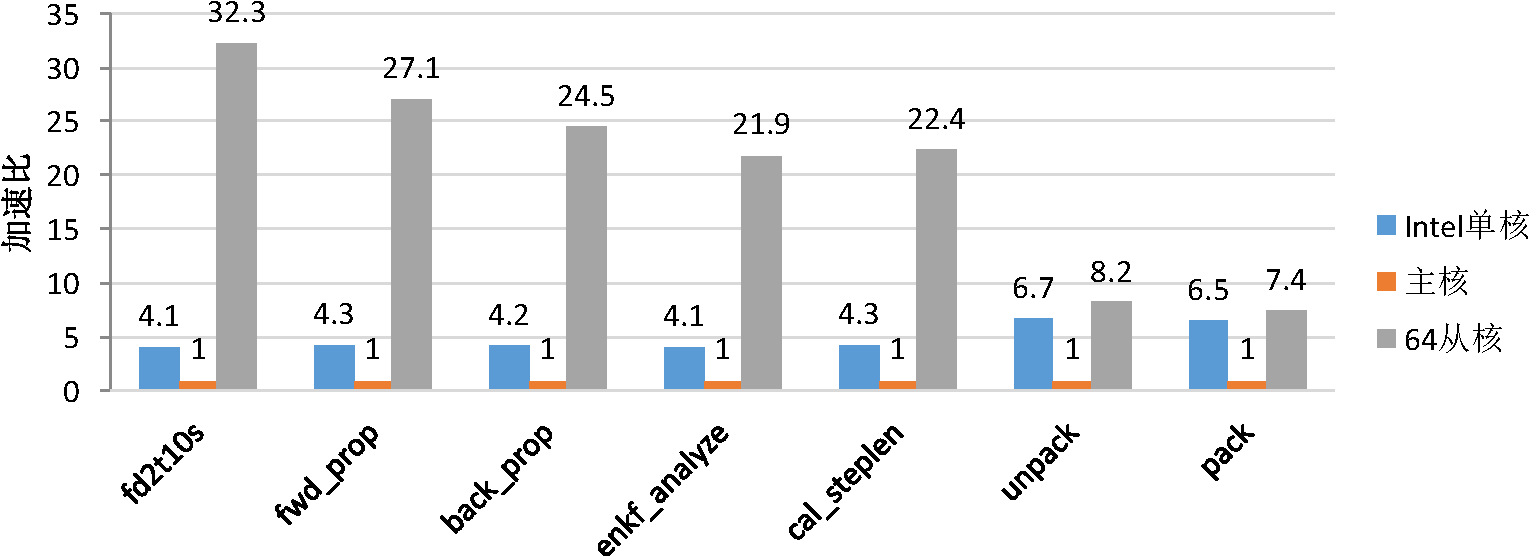
\includegraphics[width=0.9\columnwidth]{enfwi不同函数优化加速比-crop.pdf}
\caption{集合全波形反演算法核心函数从核优化加速比。}
\label{fig:集合全波形反演算法核心函数从核优化加速比}
\end{figure}


\subsection{数值实验模拟}
本小节使用数值实验模拟,比较传统全波形反演算法、震源编码全波形反演方法和集合全波形反演算法在叫不精确的初始速度模型以及有噪音的数据下的收敛情况。验证集合全波形反演方法有较大的收敛域和较小的数据噪音敏感度。

本算例中,我们对Marmousi模型进行反演,Marmousi模型是典型的二维全波形反演模型,为了使用该模型进行三维集合全波形反演,我们人为地将二维平面扩展成三维,扩展后的模型的大小为$9.2km\times 3.0km \times 5km$,空间步长为$10m$,网格的大小为$920\times 300 \times 500$。我们将震源放置在深度为$10m$的平面,在平面上每个$100m$放置一个震源,震源函数为
\begin{equation}
  f(t)=\sin(2\pi f_0t)\cdot e^{-4\pi^2f_0^2t^2/16}
\end{equation}
其中主频$f_0$为10Hz,$t$为时间。地震记录接收器(检波器)同样铺放在深度为$10m$的平面,且每个$10m$放置一个检波器,检波器铺满整个平面网格。正演的时长为$3s$。伪三维Marmousi模型正演反演数值模拟参数如表\ref{tb:伪三维Marmousi模型正演反演数值模拟参数}所示。

\begin{table}[ht]
\centering
\caption{伪三维Marmousi模型正演反演数值模拟参数}
\label{tb:伪三维Marmousi模型正演反演数值模拟参数}
\begin{tabular}{cccccc}
\hline
参数 & 反演范围($km^3$) & 分辨率 & 网格大小        & 震源频率 & 正演时长 \\\hline
配置 & 9.2*3.0*5     & 10m   & 920*300*500   & 10Hz    & 3s  \\\hline
\end{tabular}
\end{table}

Marmousi的精确速度模型如图\ref{fig:Marmousi精确模型}所示。我们使用精确速度模型进行正演得到实际观测地震记录,然后我们在精确速度模型的慢度域进行模糊化处理,平滑的窗口的大小为为$1.8km\times 0.5km$,平滑后的模型如图\ref{fig:Marmousi模型慢域平滑后的初始模型}所示。平滑后的模型(即初始速度模型)和实际观测地震记录作为集合全波形反演的输入,目标是经过300次迭代步之后,将初速速度模型反演逼近得到如图\ref{fig:Marmousi精确模型}所示的精确速度模型。

\begin{figure}[ht]
    \centering
    \begin{subfigure}[b]{0.5\textwidth}
        \centering
        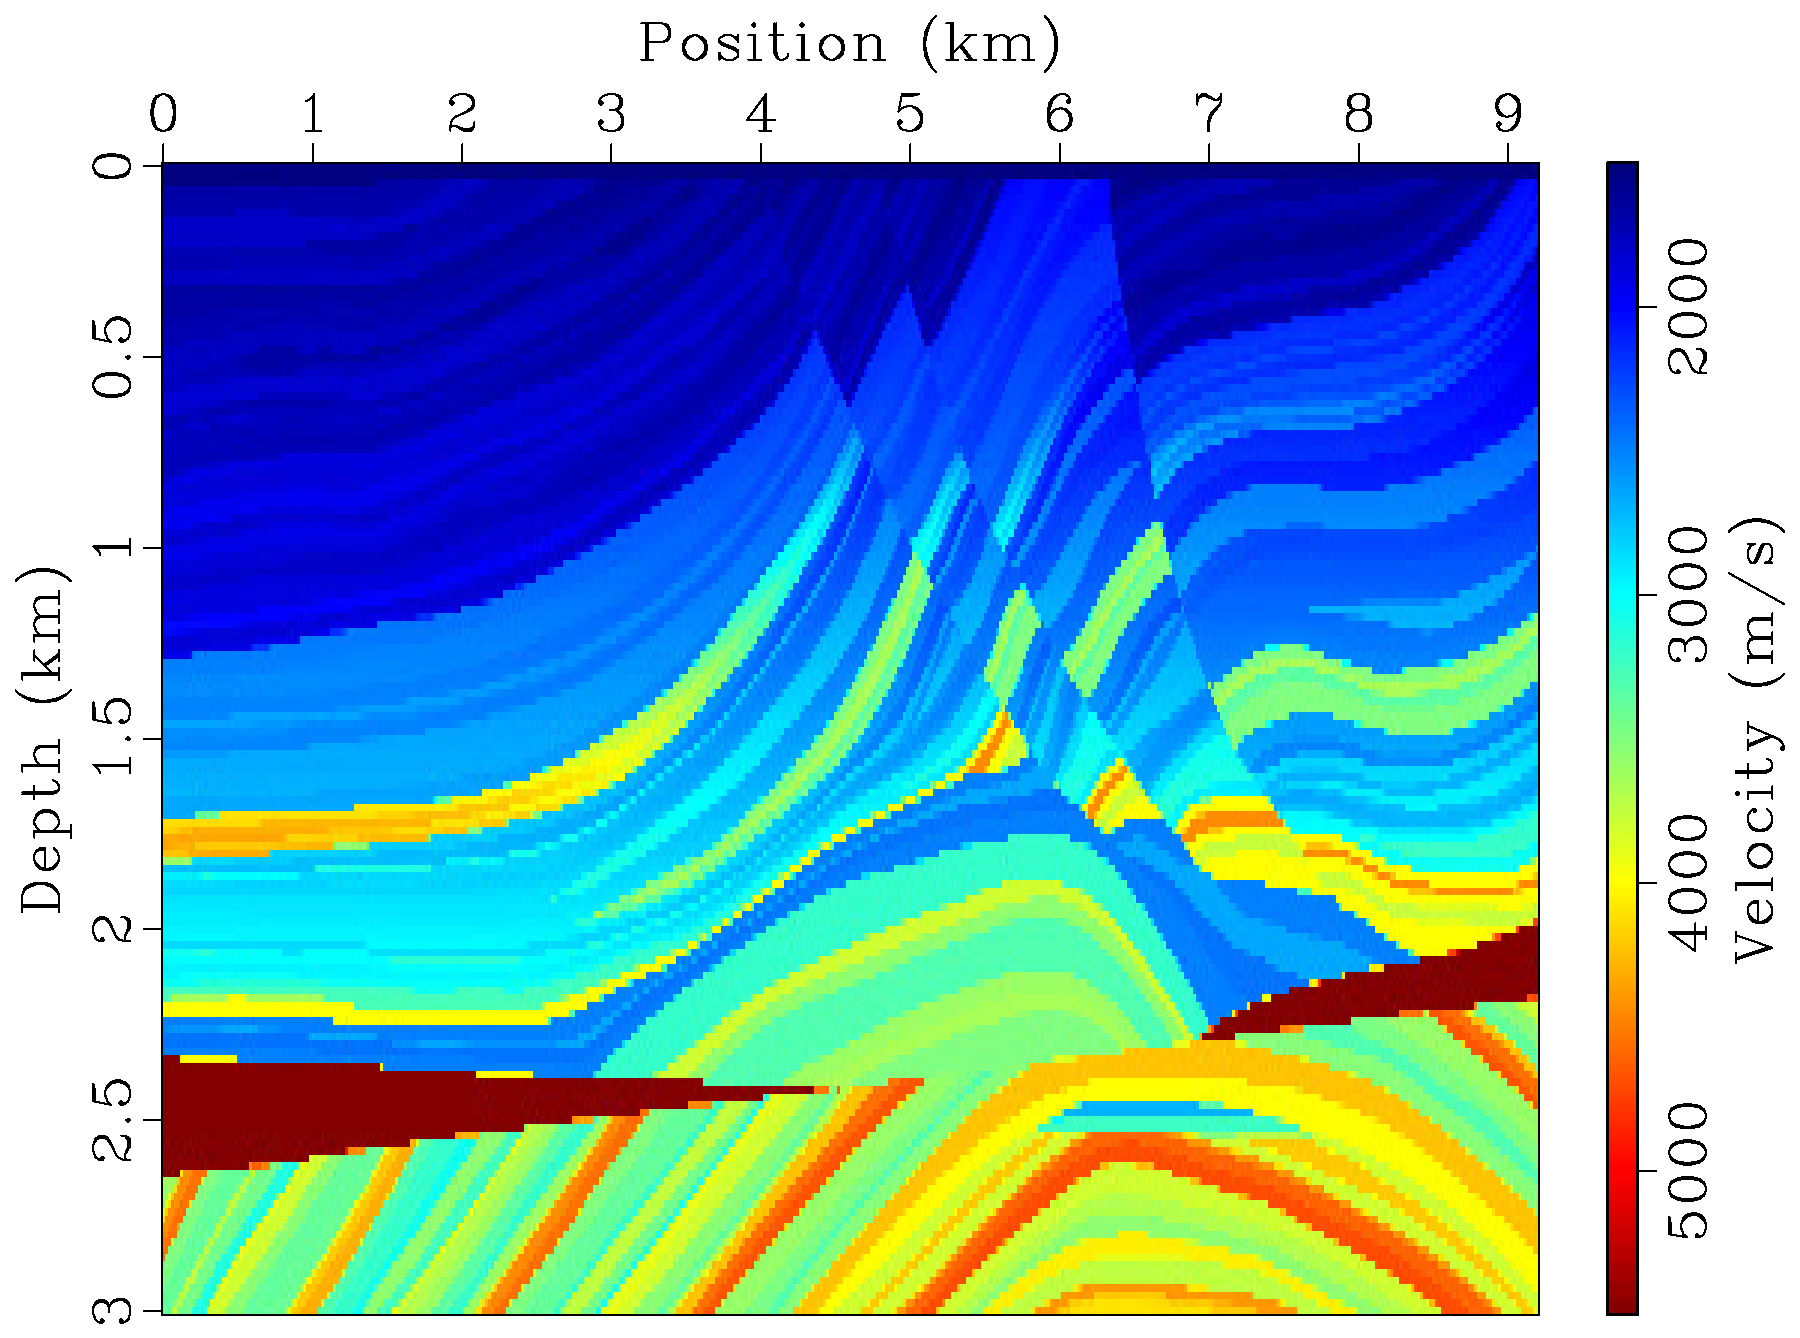
\includegraphics[height=2.1in]{marmvel.pdf}
        \caption{Marmousi精确模型。}
        \label{fig:Marmousi精确模型}
    \end{subfigure}%
    ~
    \begin{subfigure}[b]{0.5\textwidth}
        \centering
        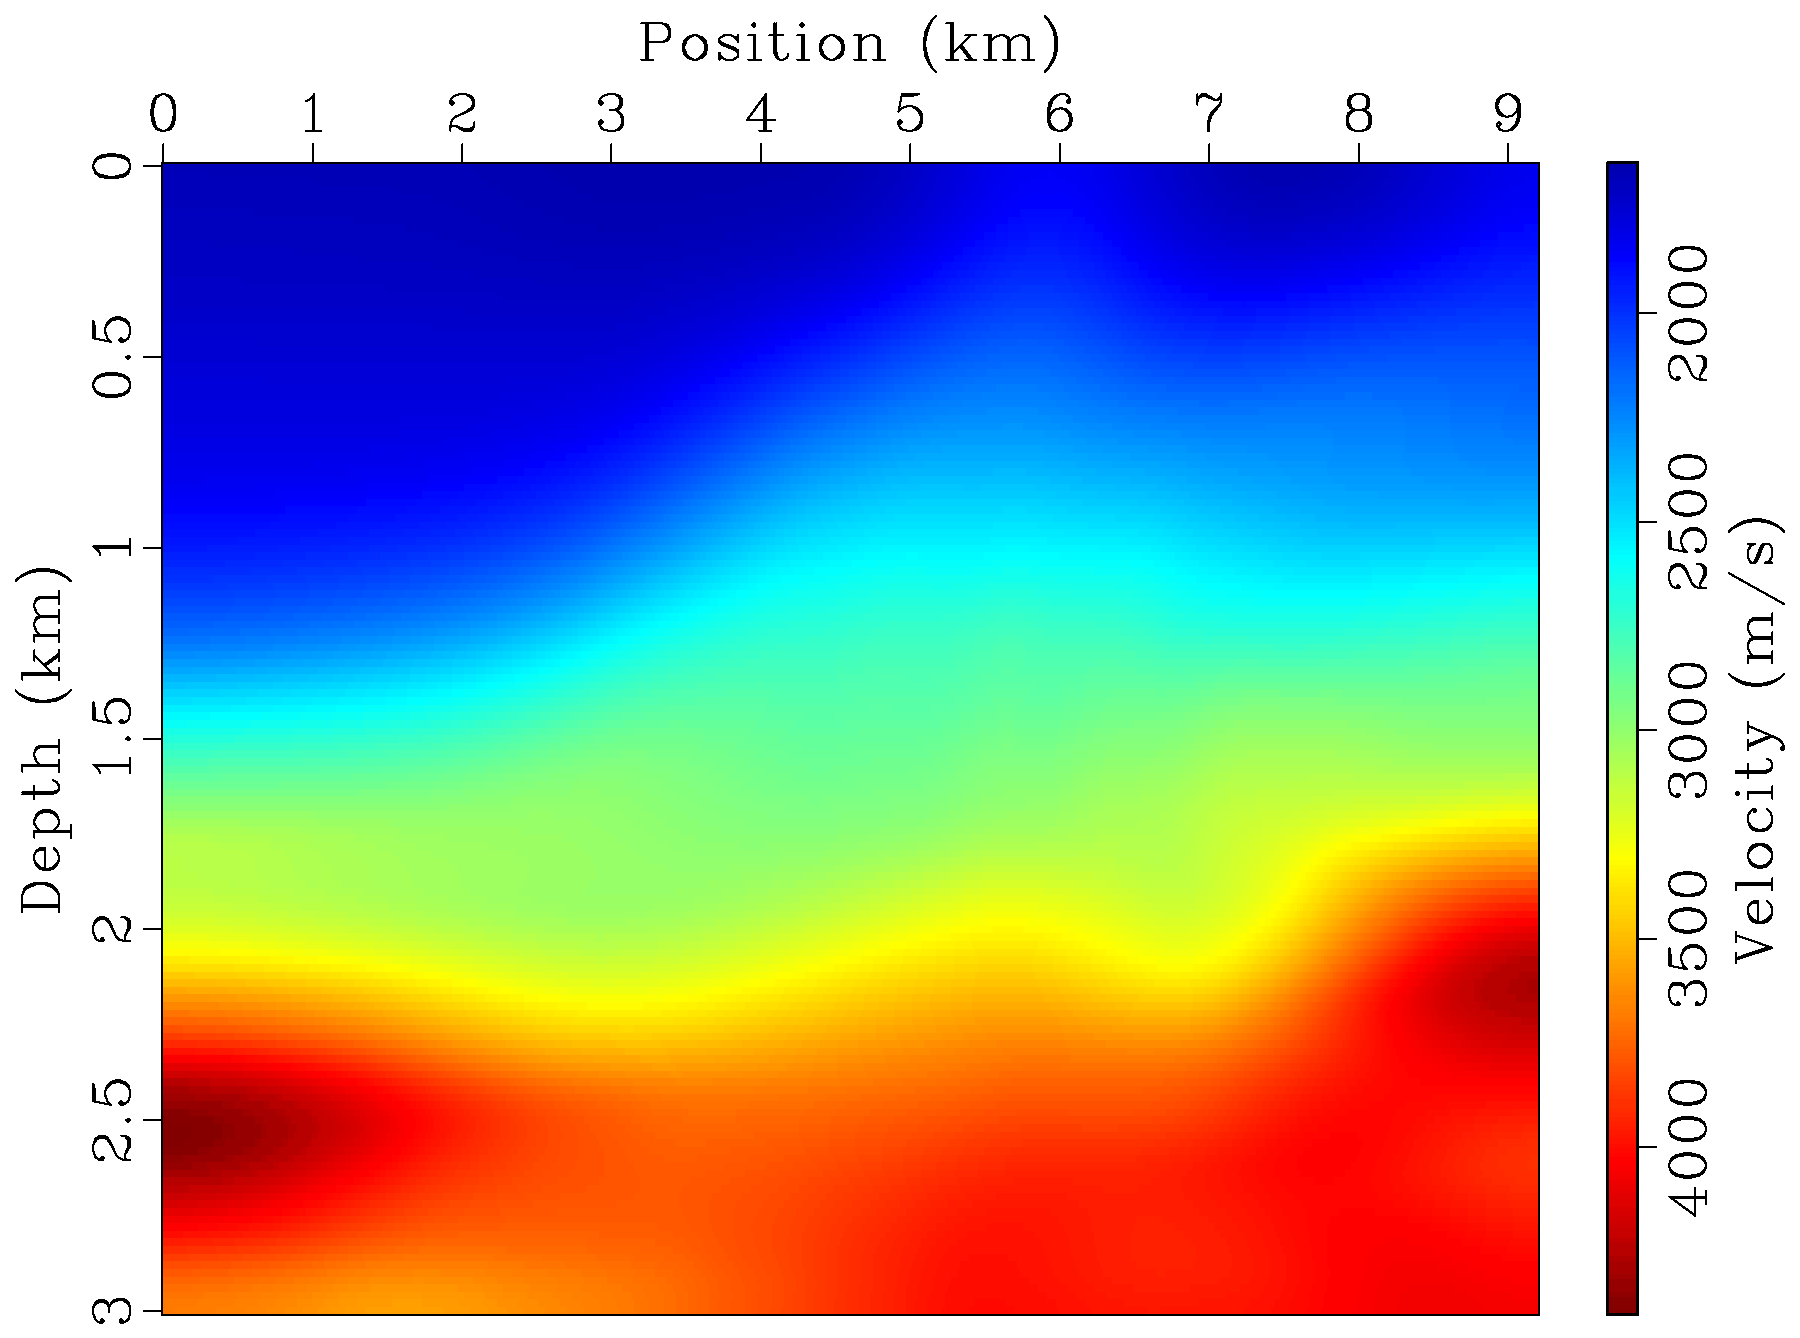
\includegraphics[height=2.1in]{marmvel_smoothed.pdf}
        \caption{Marmousi模型慢域平滑后的初始模型。}
        \label{fig:Marmousi模型慢域平滑后的初始模型}
    \end{subfigure}
    \caption{Marmousi精确模型和平滑后的初始模型}
    \label{fig:Marmousi精确模型和平滑后的初始模型}
\end{figure}


\begin{figure}[ht]
    \centering
    \begin{subfigure}[b]{0.5\textwidth}
        \centering
        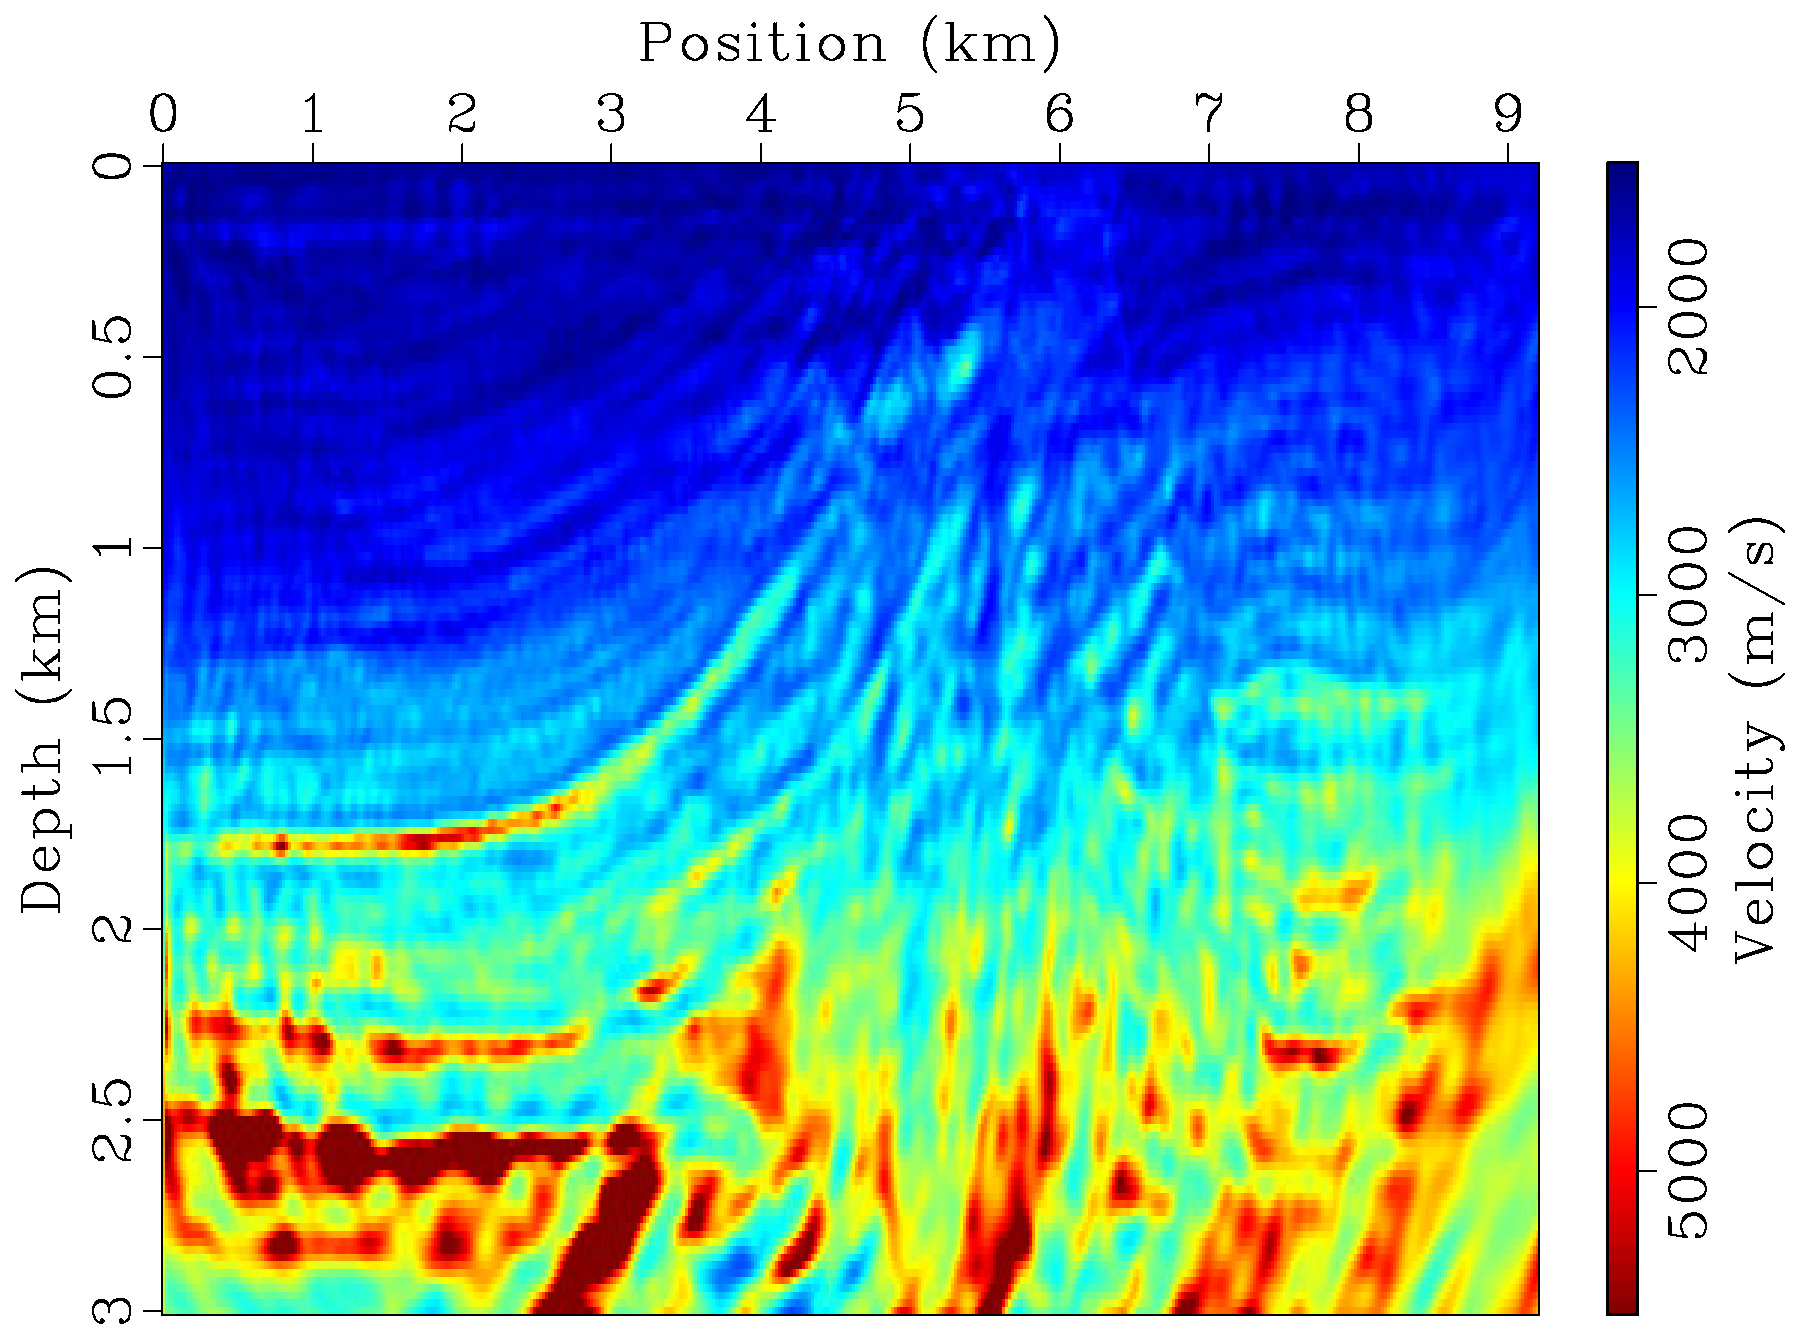
\includegraphics[height=2.1in]{fwi.pdf}
        \caption{无噪音全波形反演结果。}
        \label{fig:无噪音全波形反演结果}
    \end{subfigure}%
    ~
    \begin{subfigure}[b]{0.5\textwidth}
        \centering
        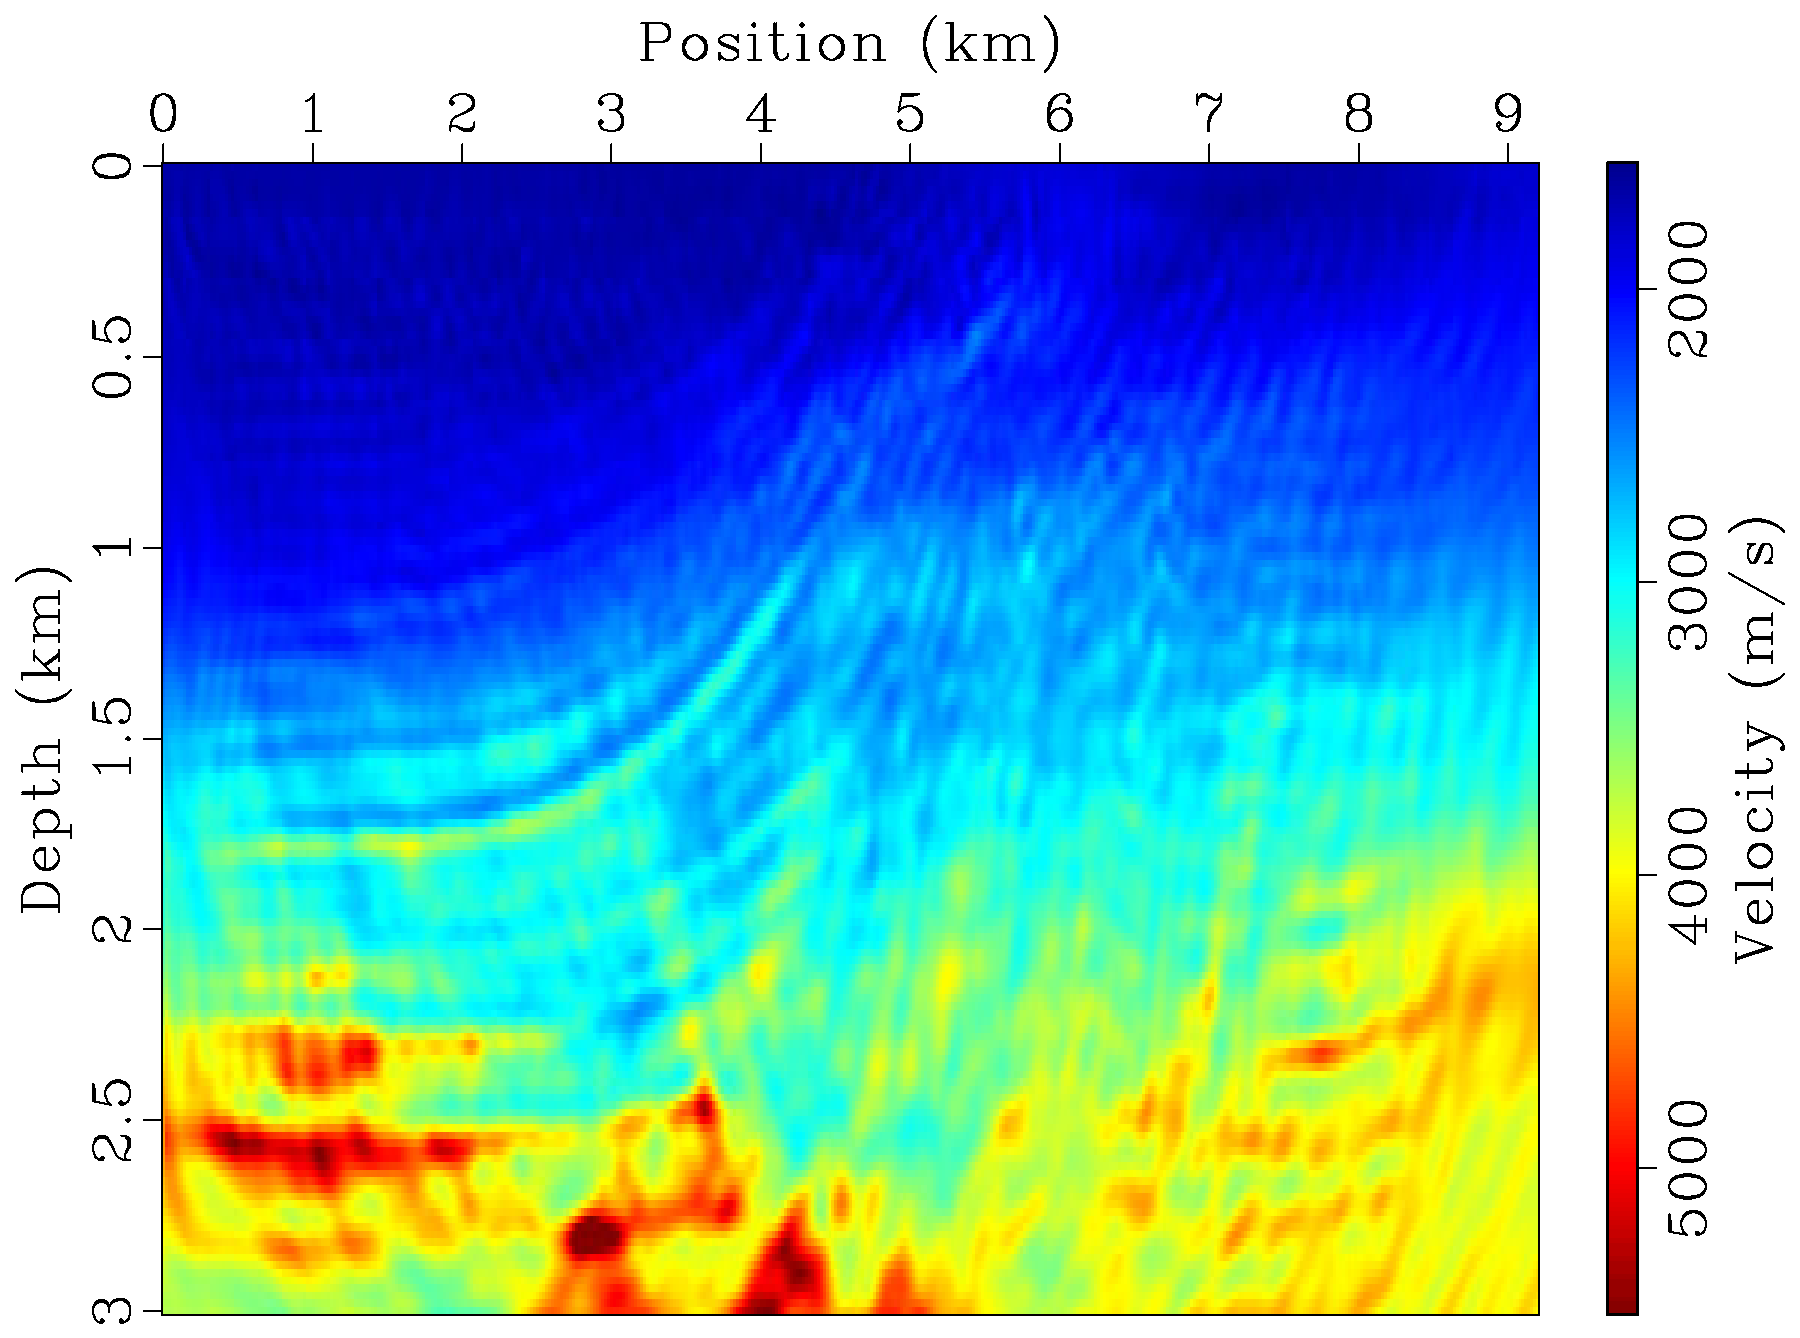
\includegraphics[height=2.1in]{fwi-noise.pdf}
        \caption{有噪音全波形反演结果。}
        \label{fig:有噪音全波形反演结果}
    \end{subfigure}
    \caption{传统全波形反演在无噪音和有噪音情况下的反演成像结果。}
\end{figure}

\begin{figure}[ht]
    \begin{subfigure}[b]{0.5\textwidth}
        \centering
        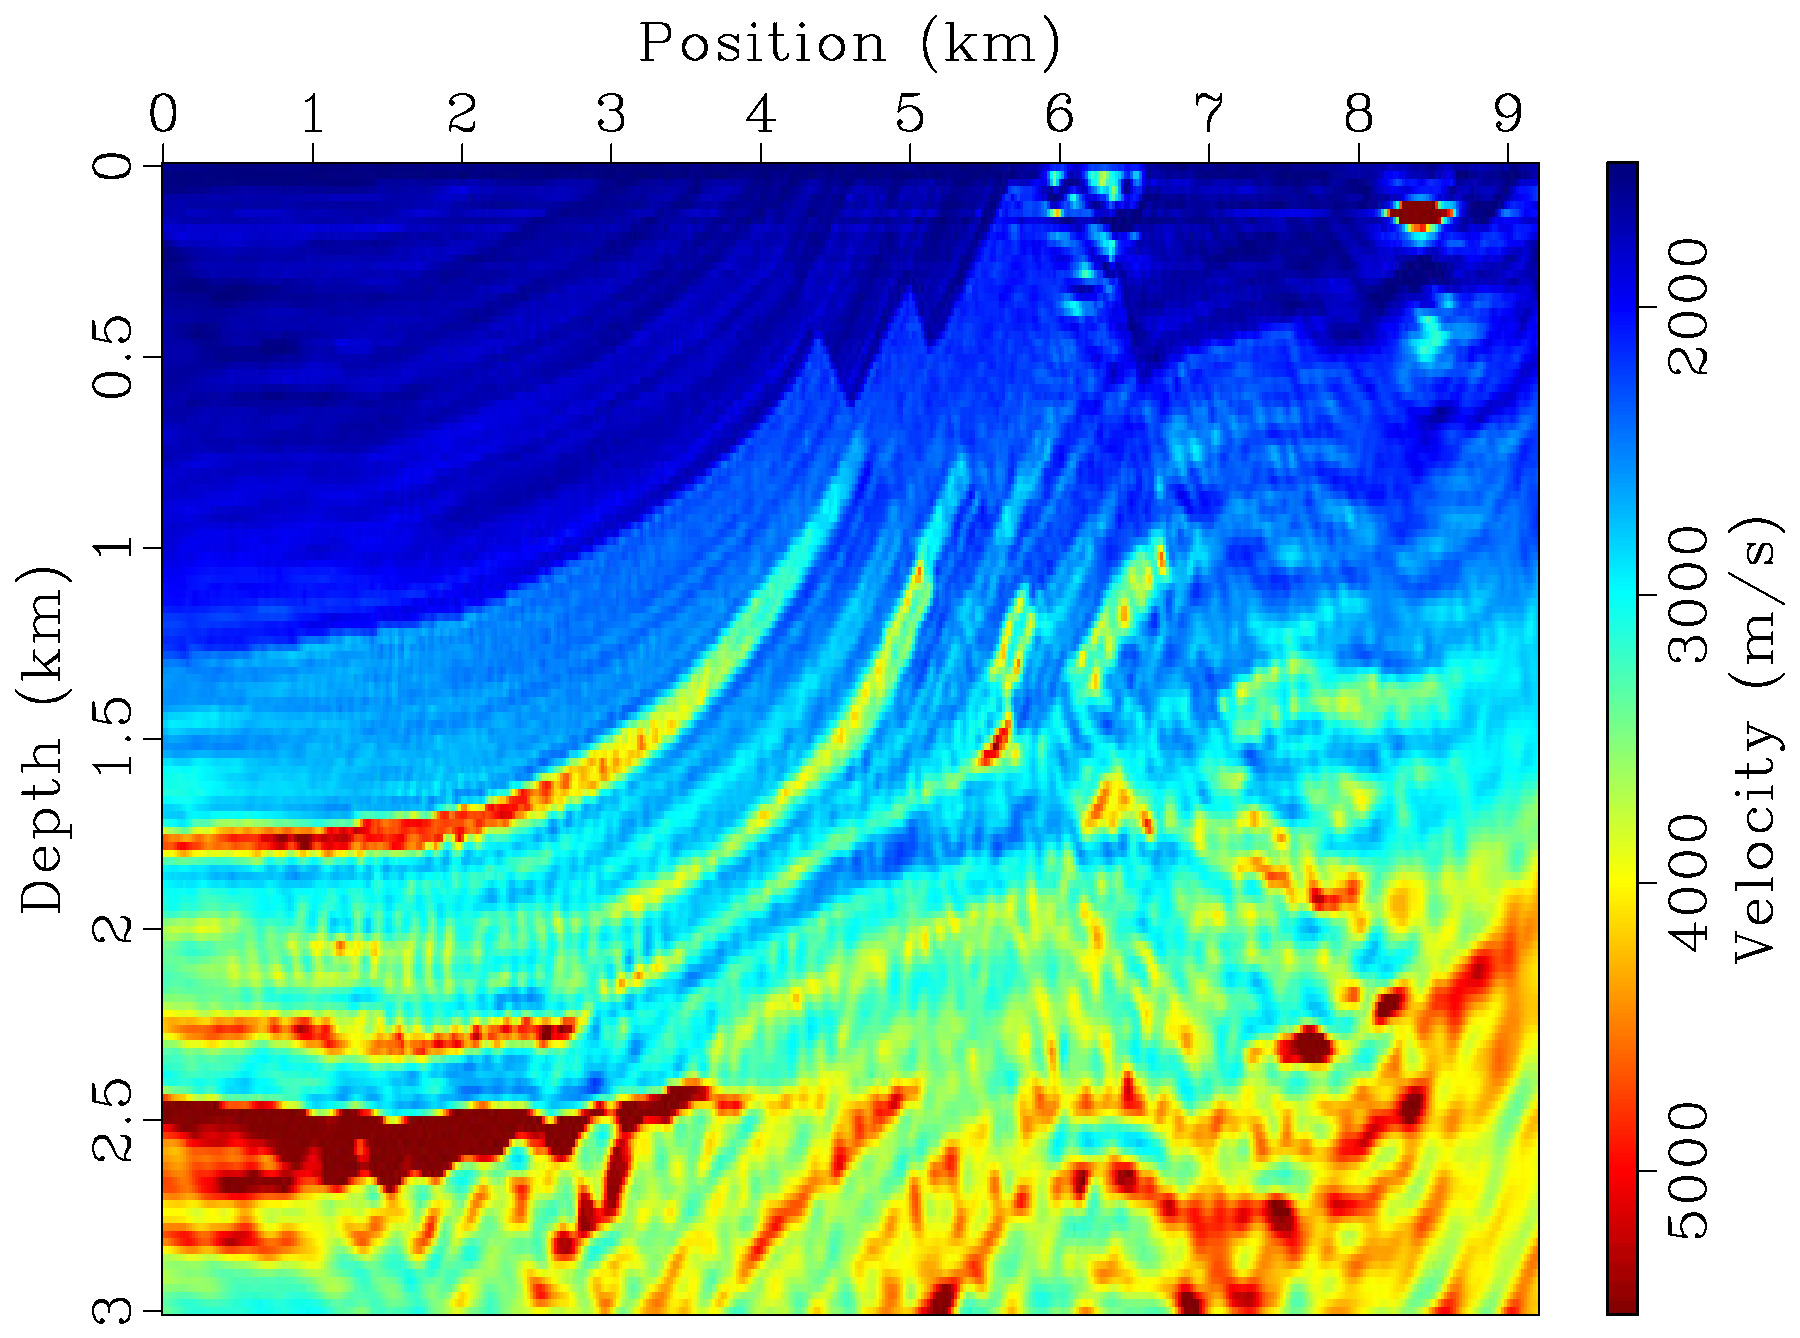
\includegraphics[height=2.1in]{esfwi.pdf}
        \caption{无噪音震源编码全波形反演结果。}
        \label{fig:无噪音震源编码全波形反演结果}
    \end{subfigure}%
    ~
    \begin{subfigure}[b]{0.5\textwidth}
        \centering
        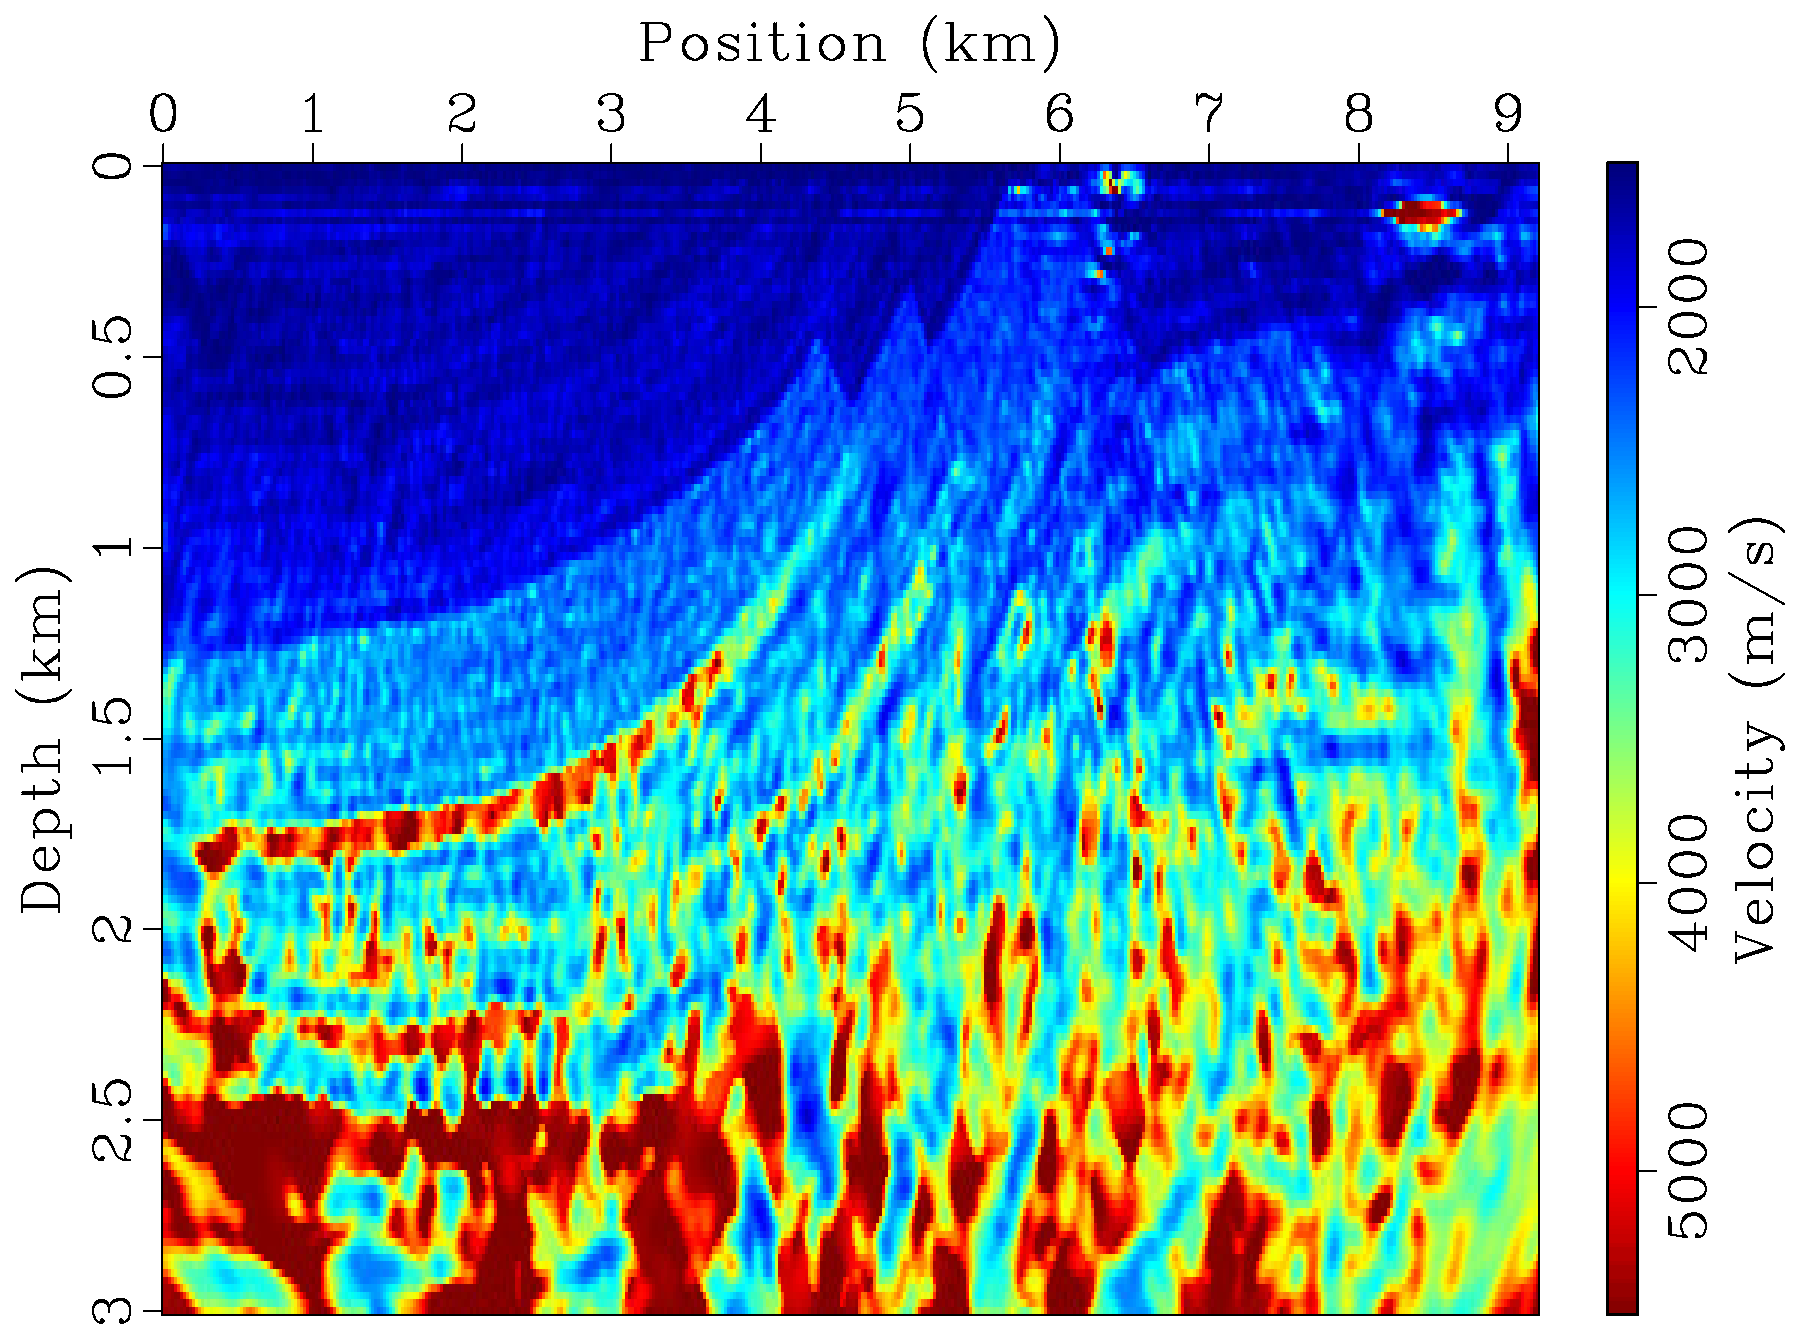
\includegraphics[height=2.1in]{esfwi-noise.pdf}
        \caption{有噪音震源编码全波形反演结果。}
        \label{fig:有噪音震源编码全波形反演结果}
    \end{subfigure}
    \caption{震源编码全波形反演在无噪音和有噪音情况下的反演成像结果。}
\end{figure}

\begin{figure}[ht]
    \begin{subfigure}[b]{0.5\textwidth}
        \centering
        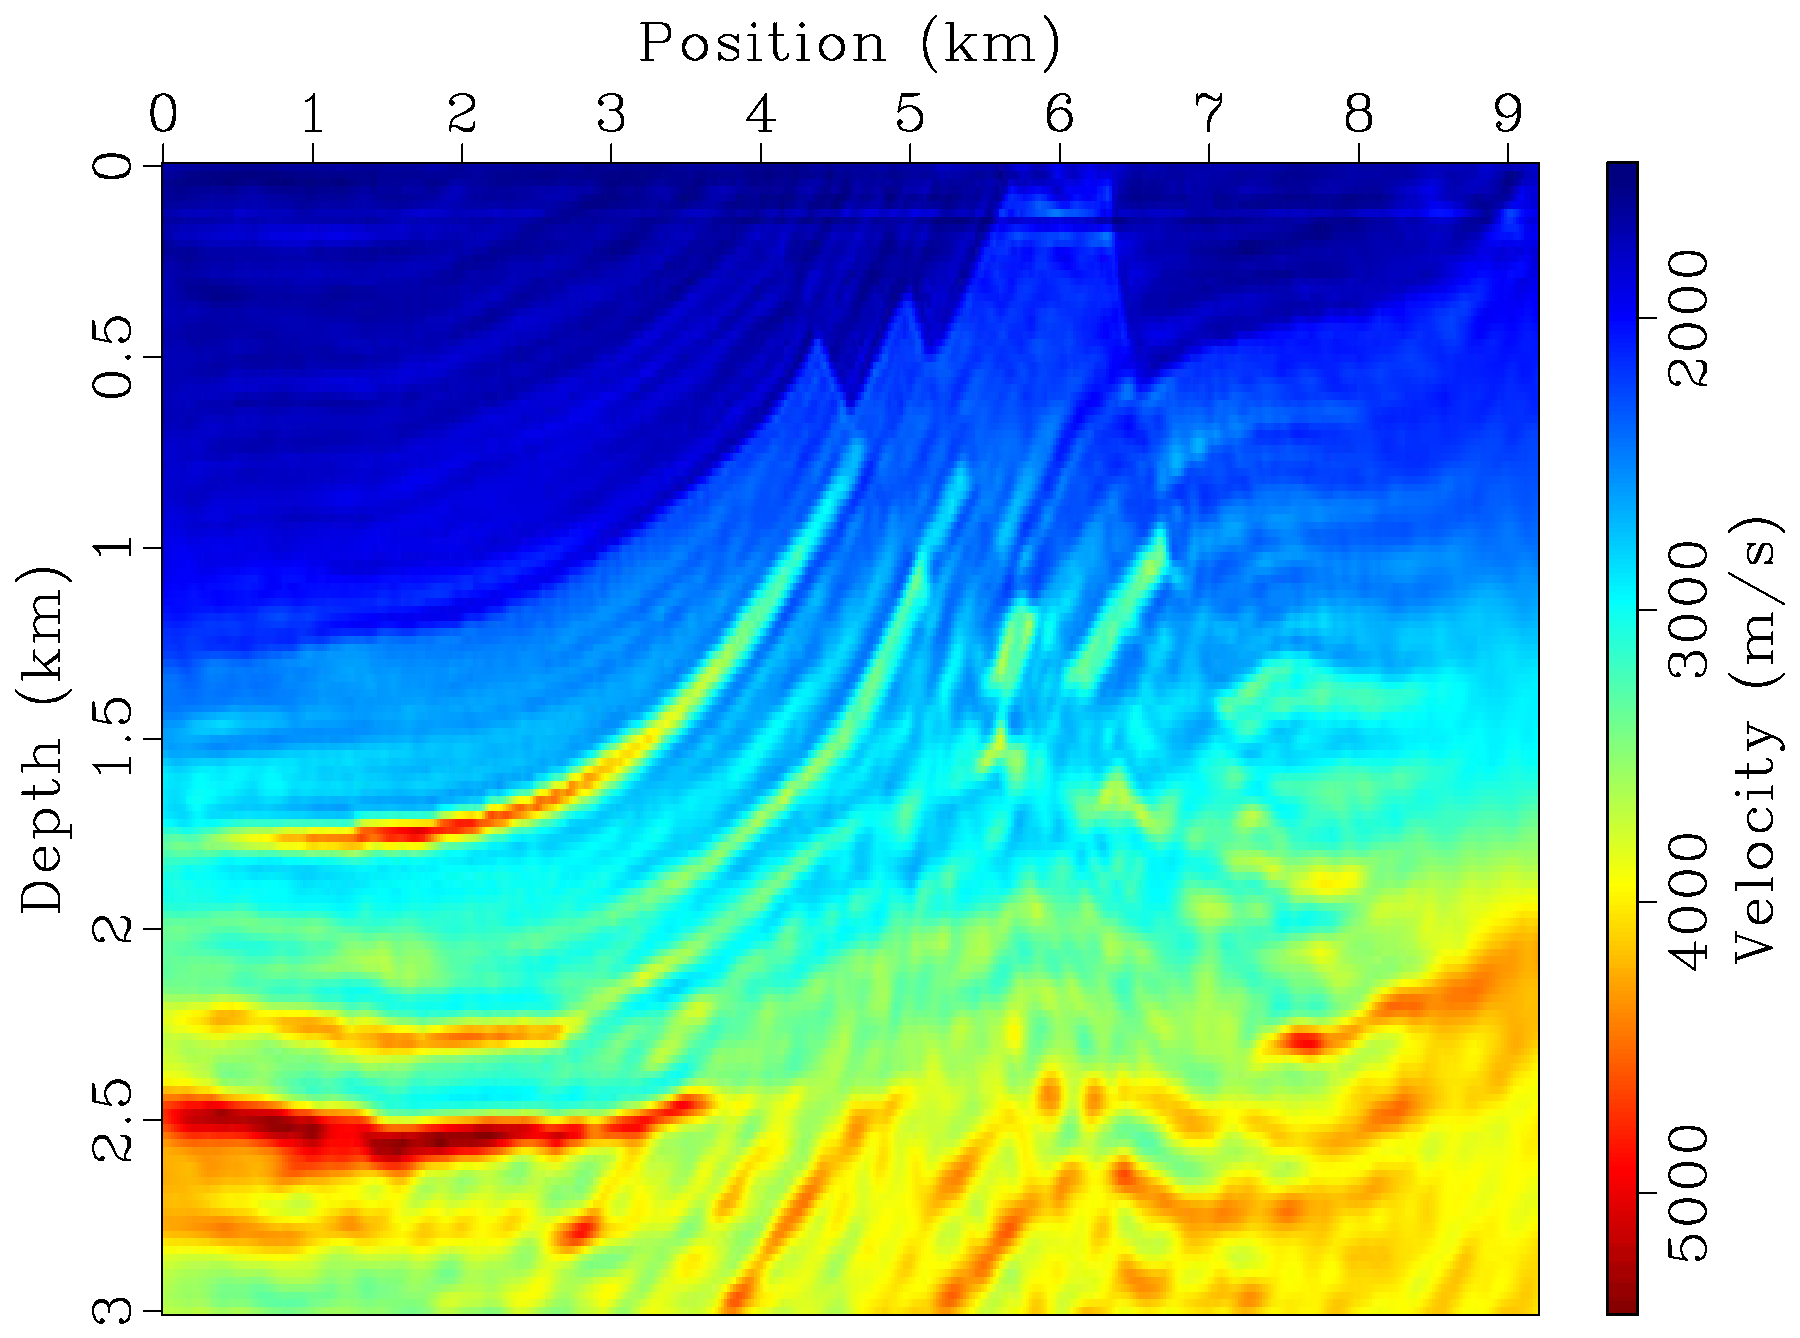
\includegraphics[height=2.1in]{enfwi.pdf}
        \caption{无噪音集合全波形反演结果。}
        \label{fig:无噪音集合全波形反演结果}
    \end{subfigure}%
    ~
    \begin{subfigure}[b]{0.5\textwidth}
        \centering
        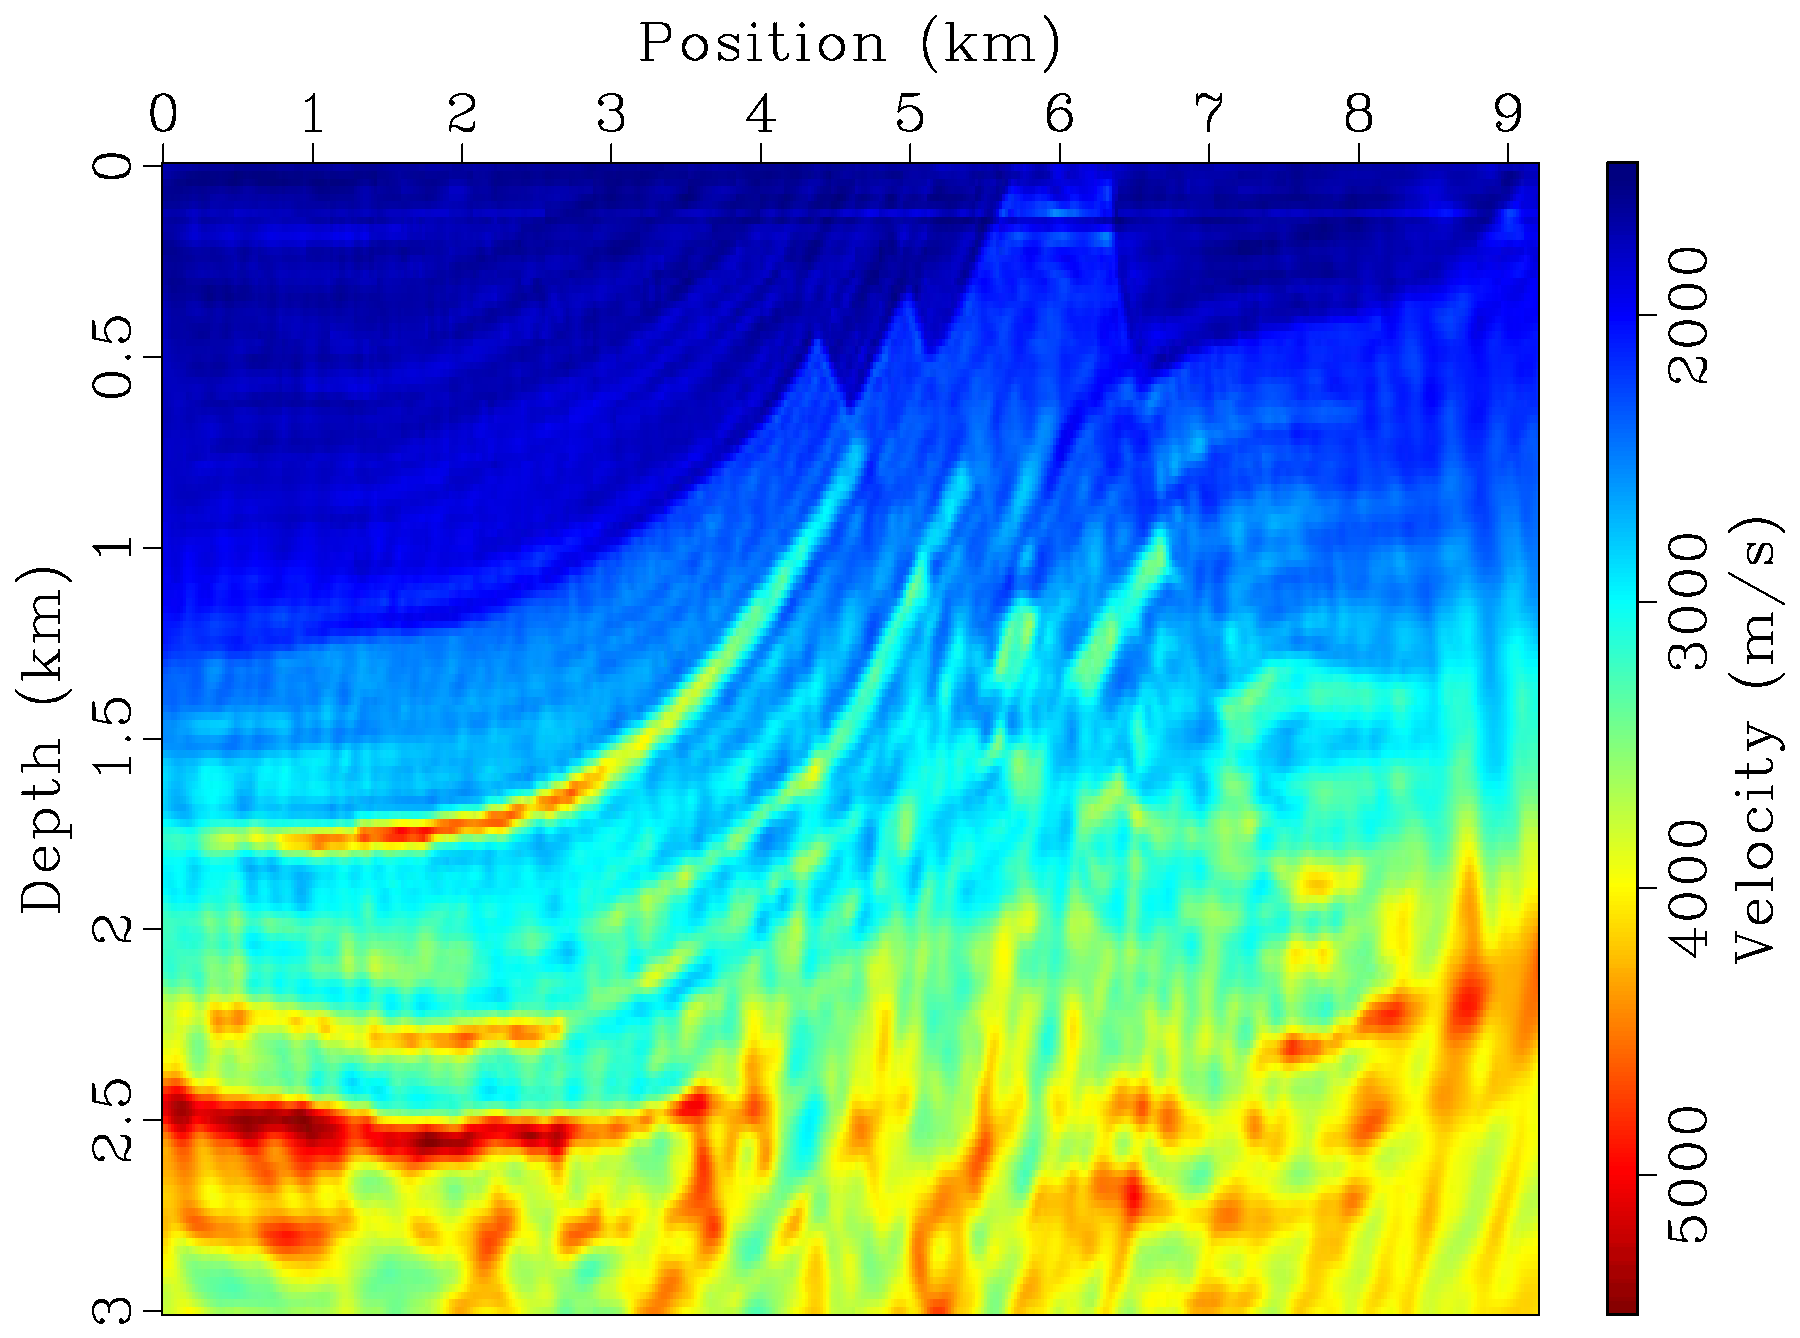
\includegraphics[height=2.1in]{enfwi-noise.pdf}
        \caption{有噪音集合全波形反演结果。}
        \label{fig:有噪音集合全波形反演结果}
    \end{subfigure}
    \caption{集合全波形反演在无噪音和有噪音情况下的反演成像结果。}
\end{figure}

图\ref{fig:无噪音全波形反演结果}、\ref{fig:无噪音震源编码全波形反演结果}、\ref{fig:无噪音集合全波形反演结果}分别描述了无噪音情况下全波形反演、震源编码全波形反演、集合全波形反演算法的成像结果。我们可以看到,在初始模型较差的情况下,传统全波形反演算法只能勾画出大致的速度层状结构,但缺乏高频信息;震源编码全波形反演结果能够反演出较好的层状结构,尤其是在低速区,反演的结果几乎与真实模型相同,但也陷入了局部最优(如图\ref{fig:无噪音震源编码全波形反演结果}右上角红点所示)。集合全波形反演算法克服了全波形反演和震源编码全波形反演算法的不足,清晰的反演出最接近真实的速度模型。在高速区域的反演效果明显好于前两种算法。此外,由于全波形反演算法最终对所有样本基本进行均值化处理,最终反演的速度模型有明显的平滑效果,消除了局部最优的假象。

我们在观测地震记录中加入了幅值为全局地震记录最大值的5\%的白噪音。在较差的初始速度模型和数据噪音的双重影响下,图\ref{fig:有噪音全波形反演结果}、\ref{fig:有噪音震源编码全波形反演结果}、\ref{fig:有噪音集合全波形反演结果}分别描述了无噪音情况下全波形反演、震源编码全波形反演、集合全波形反演算法的成像结果。我们可以看到,在有噪音情况下,三种方法的成像效果都不理想。传统的全波形反演算法几乎无法勾勒出Marmousi模型的大致结构,只有少量的有效信息。震源编码全波形反演算法对数据噪音最敏感,出现了大量的人工假象。而集合全波形反演较有效地克服了数据噪音,在低速区反演出精确的模型,在高速区也较好的对抗了噪音造成的影响。

由此可见,集合全波形算法与传统全波形反演、震源编码全波形反演具有更大的收敛域,且对数据噪音更不敏感。在处理的地震成像中具有更大的应用潜力。

\section{本章小结}

本章以真实的地震模拟算例为背景,应用前文所述的地震模拟并行优化方法,展现了唐山大地震和石油物探全波形反演算法在神威太湖之光上取得的性能提升以及模拟结果。非线性唐山大地震模拟使用了神威超算千万核心,模拟范围达到了$320km\times 320km \times 40km$,分辨率高达$8m$,频率高达$18Hz$,峰值性能达到18.9 PFlops,这是迄今为止最大规模、最高分辨率的地震模拟。随后,本研究在高效正演的基础上使用了集合全波形反演算法反演了石油物探的Marmousi模型,借助神威超算系统的各项资源优势,取得了良好的性能结果。反演结果显示,集合全波形反演算法与传统全波形反演方法和基于震源编码的全波形反演方法相比具有更大的收敛域和更低的噪音敏感度。
